\section{问题一的模型建立与求解}

\subsection{问题分析}

问题一要求完成三项任务：（1）建立数据质量评分方法，给出样本级与域级质量分；
（2）定义并消解质量信号冲突；（3）建立 17 领域配比与损失之间的数量关系模型，
并讨论配比效应随规模的转移。A1--A3 提供约 27.3 万条样本、22 个质量指标
（14 项标量、8 项列表型），A4--A15 提供 1M/60M/1B 训练集与 10b/70b 估计
五档规模下的配比--损失数据，A16 给出 17 个配比域到 7 个质量域的映射。

\subsection{质量评分模型}

\subsubsection{指标预处理}

质量指标分为标量指标（如词数、熵、可读性等）与列表型指标（如各质量模型的
得分分布）。列表型指标先取均值压缩为标量；对``数值越小越好''的负向指标
（如无字母词占比、重复率）取相反数统一方向；随后对各指标做 1\%/99\% 缩尾
抑制离群值，再按 Min--Max 归一化到 $[0,1]$。经处理后得到标准化指标矩阵
$X\in[0,1]^{n\times 22}$。

\subsubsection{组合赋权}

为避免单一赋权法的偏差，采用熵权法与 CRITIC 法按 $0.5:0.5$ 组合：
\begin{equation}
w_j=\frac{1}{2}w_j^{\text{ent}}+\frac{1}{2}w_j^{\text{critic}},\qquad
w_j^{\text{ent}}=\frac{1-H_j}{22-\sum_k H_k},\quad
w_j^{\text{critic}}=\frac{\sigma_j\sum_{k\neq j}(1-|r_{jk}|)}{\sum_l
\sigma_l\sum_{k\neq l}(1-|r_{lk}|)}
\label{eq:weights}
\end{equation}
其中 $H_j$ 为第 $j$ 指标的归一化信息熵，$r_{jk}$ 为指标间 Spearman 相关系数。
熵权法强调信息量，CRITIC 强调指标强度与独立性，二者互补。

\subsubsection{TOPSIS 综合评分}

在组合权重下构造加权标准化矩阵 $V_{ij}=w_j X_{ij}$，计算正理想解
$V^{+}$（各列最大值）与负理想解 $V^{-}$（各列最小值），样本质量分为贴近度：
\begin{equation}
Q_i=\frac{d_i^{-}}{d_i^{+}+d_i^{-}},\qquad
d_i^{+}=\sqrt{\sum_j (V_{ij}-V_j^{+})^2},\quad
d_i^{-}=\sqrt{\sum_j (V_{ij}-V_j^{-})^2}.
\label{eq:topsis}
\end{equation}
$Q_i\in[0,1]$，越接近 1 质量越高。域级质量按样本加权平均聚合：
$Q^{(d)}=\sum_{i\in d}w_i Q_i/\sum_{i\in d}w_i$。

\textbf{评分方法一致性}（图 \ref{fig:p1_methods}）：在相同预处理数据上
（A1 抽样集 + A2/A3 扩展集，$n=81{,}230$）用\textbf{八种评分方法}——加权
聚合类（TOPSIS、SAW 加权和、熵-CRITIC 加权、CRITIC-only）、灰色关联
GRA、秩和比 RSR，以及标准多准则决策框架 PROMETHEE-II（outranking 净
流量 $\phi^{+}-\phi^{-}$）与 VIKOR（折衷解 $Q=vS+(1-v)R$）——分别得到
七域域级排序。结果：加权/贴近度/折衷五方法（TOPSIS、SAW、熵-CRITIC、
PROMETHEE-II、VIKOR）域序\textbf{高度一致}，两两 Spearman 最小 0.93、
均值 0.97；其中 TOPSIS/SAW/熵-CRITIC/PROMETHEE-II 四方法域序\textbf{完全
一致}（book 最优、commoncrawl 最差），VIKOR 折衷口径下仅发生两对相邻
互换（book 与 arxiv、c4 与 commoncrawl），book 稳定前二、c4/commoncrawl
稳定垫底。GRA 与加权族同为 book 居首但全序略异（arxiv 落至第 7）；纯秩法
RSR 因忽略指标幅值而偏离（book 降至第 6、wikipedia 升至第 1）。八方法
总体 Kendall 协同系数 $W=0.69$、两两 Spearman 均值 0.65（最小 0.14，
来自 GRA--VIKOR 对）——域序一致性主要来自保留幅值信息的加权/折衷族，
这也正是主链路采用``组合赋权 + TOPSIS 贴近度''的依据：秩法会丢失幅值
信息，不适合作质量评分主链路。对 $W$ 的\textbf{统计显著性}做置换检验
（随机重排 81{,}230 个样本的域标签 $B=2{,}000$ 次）：加权/贴近度/折衷
五方法的 $W=0.98$ 远在置换零分布右尾之外（零分布 95\% 分位 0.82），
置换 $p<0.001$；八方法总体 $W=0.69$ 的置换 $p=0.06$——7 个域的样本量
下该检验功效有限，且主要失分来自秩法 RSR 的偏离，再次说明``域序一致性''
显著且强地集中于加权/折衷族（$p<0.001$），秩法 RSR 是唯一系统性偏离者。

\begin{figure}[htbp]
\centering
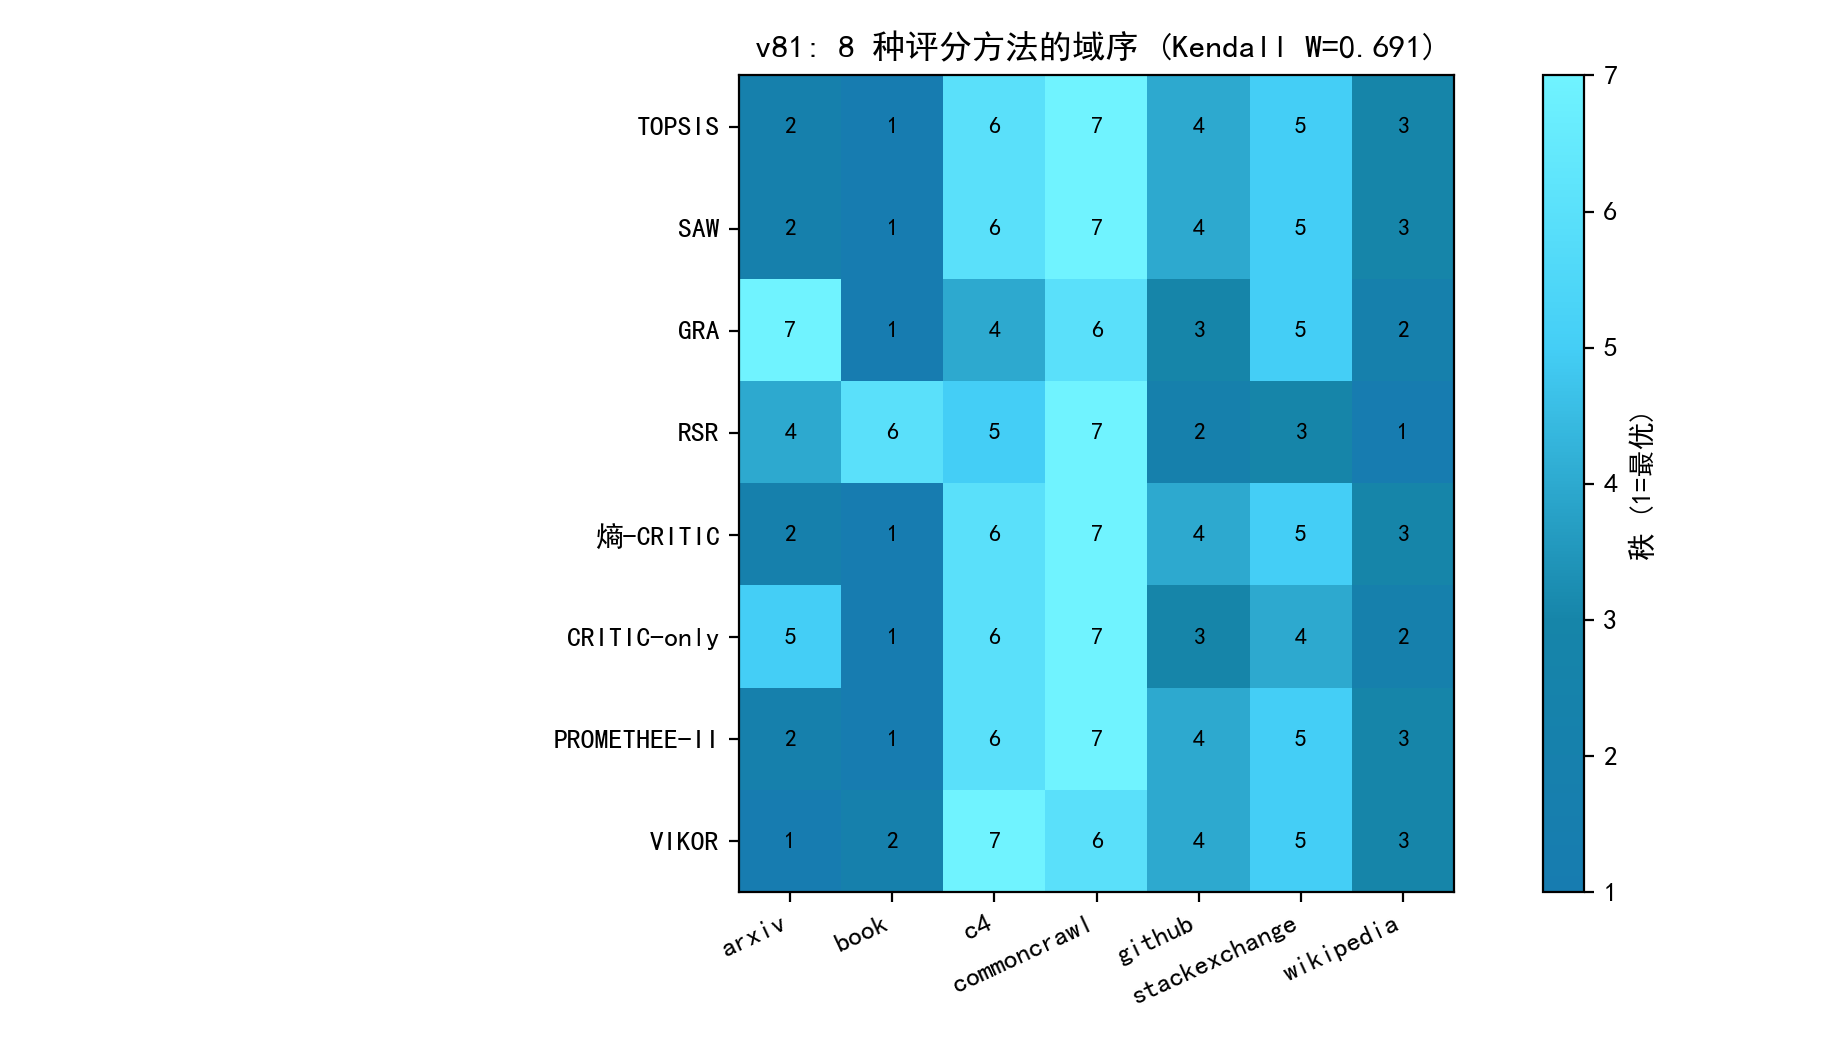
\includegraphics[width=0.85\textwidth]{figures/v81_p1_method_agree8.png}
\caption{八种评分方法的七域域序（加权/折衷五方法高度一致，秩法偏离）。}
\label{fig:p1_methods}
\end{figure}

\subsubsection{指标结构核验}

对 272{,}505 个样本的 22 项指标做数据驱动核验（图 \ref{fig:p1_family}）：
（i）\textbf{近似正交性}——指标间 Spearman 平均秩相关极低（族内
$-0.01$/$+0.02$，跨族 $-0.01$，第一主成分仅解释 37\% 方差），说明 22 项
指标各自携带独立信息，组合赋权不存在冗余放大，冲突指数
$|Q_C-Q_F|$ 具有增量信息；（ii）\textbf{族划分不可由无监督聚类恢复}——
对 $1-\rho$ 距离做层次聚类并切 2 簇，与手工族划分的调整兰德指数约 0
（样本级 $-0.02$、域级 $-0.06$）：$C/F$ 是\textbf{构念区分}（内容质量 vs
格式洁净），其效度由冲突指数的域级排序与指标族消融（灵敏度节）操作性地
支持，而非统计簇结构。该检验同时验证了手工族划分的``非数据挖掘''属性。

\begin{figure}[htbp]
\centering
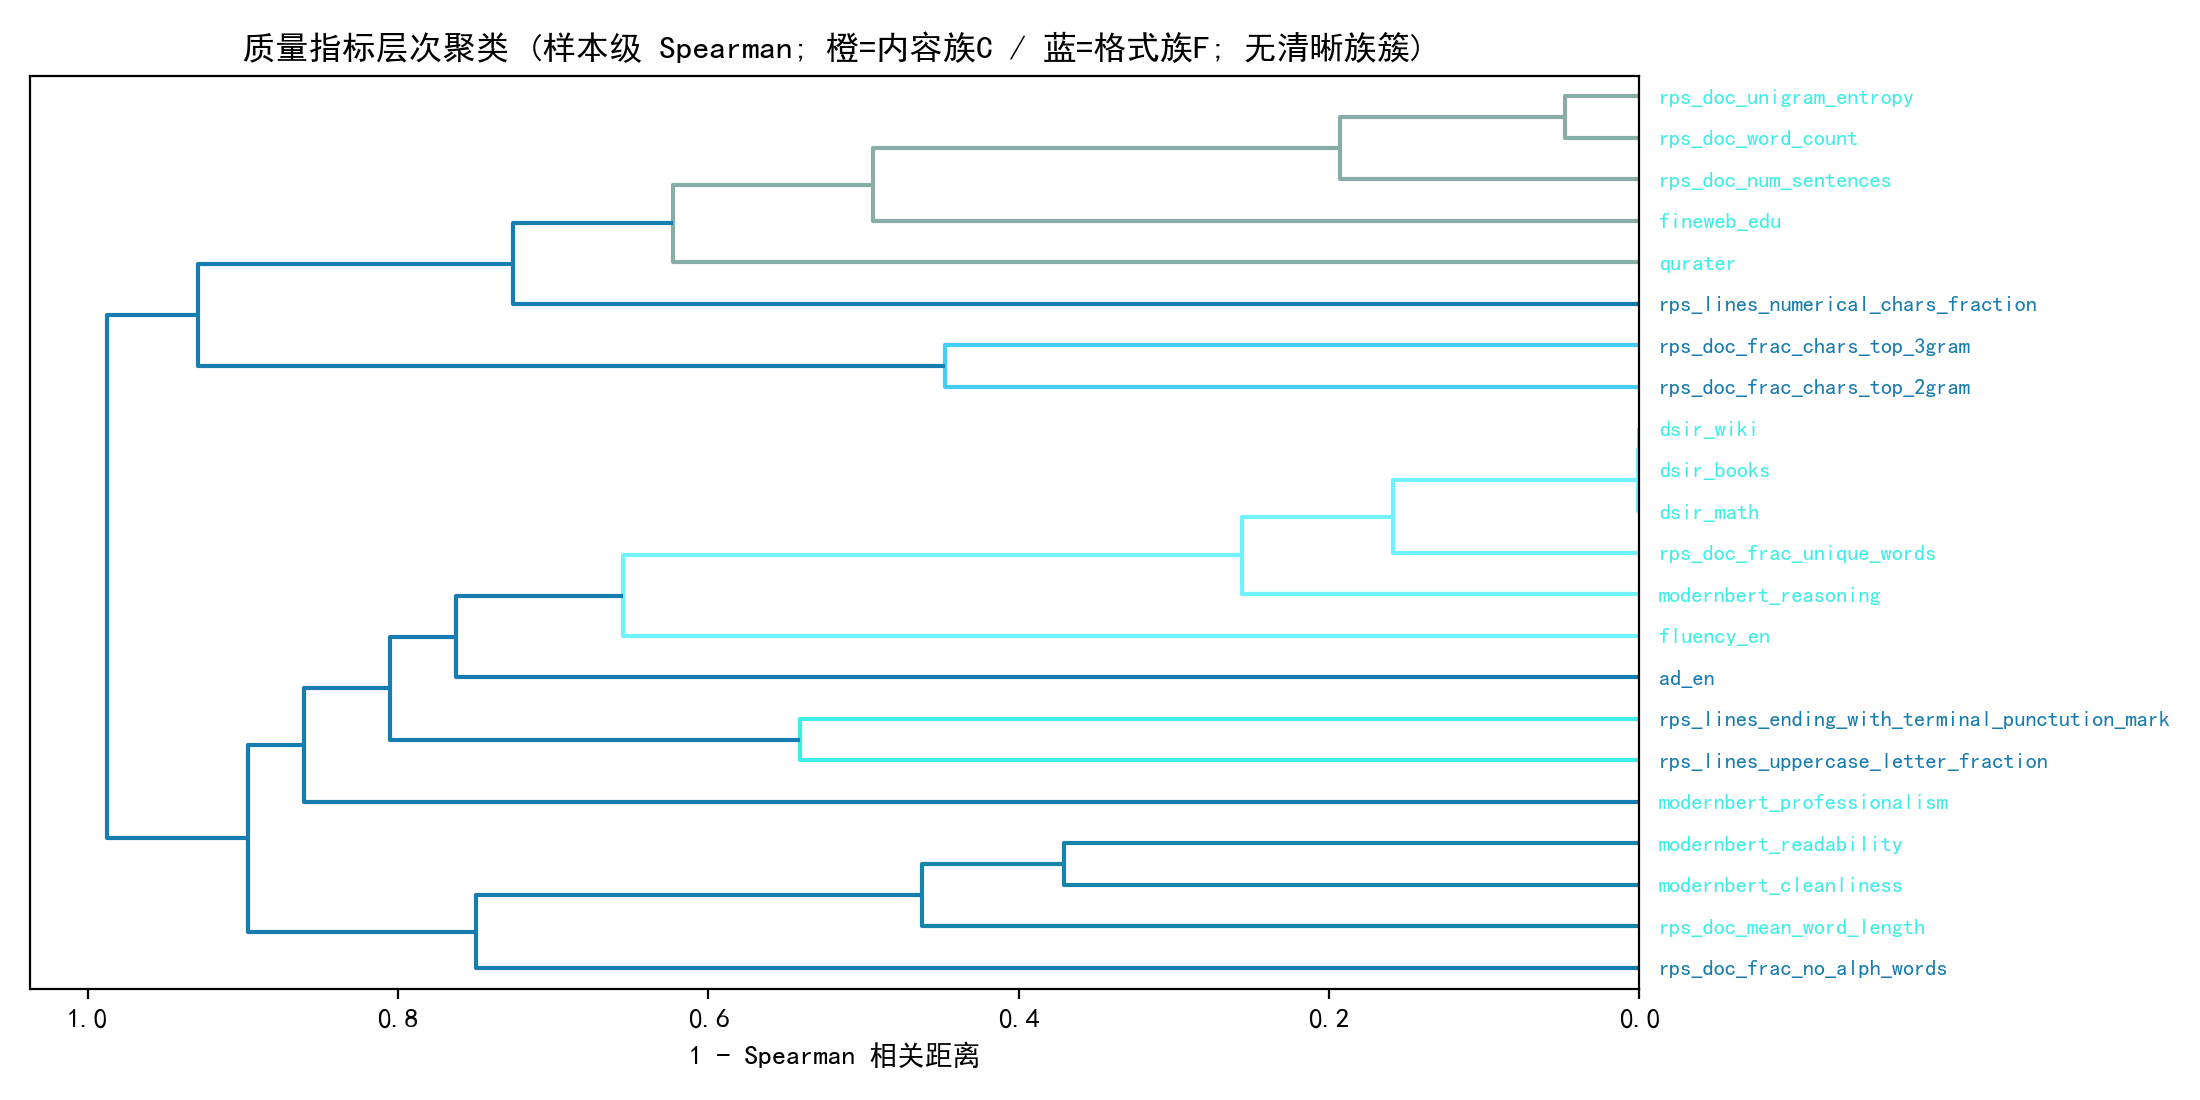
\includegraphics[width=0.9\textwidth]{figures/v21_p1_family_cluster.png}
\caption{22 项质量指标的层次聚类树状图（着色=手工族划分；无清晰族簇）。}
\label{fig:p1_family}
\end{figure}

\subsection{冲突定义与消解}

\subsubsection{双族冲突指数}

将 22 项指标划分为``内容质量族''（15 项，含各质量模型得分、推理/专业性等，
记为 $Q_C$）与``格式清洁族''（7 项，含词长、标点、无字母占比等，记为
$Q_F$）。样本级冲突指数定义为：
\begin{equation}
\mathrm{conf}_i=\bigl|Q_C(i)-Q_F(i)\bigr|,
\label{eq:conflict}
\end{equation}
它量化了``内容很好但格式脏''（或反之）的样本所呈现的信号矛盾。统计显示
冲突指数均值 0.152、最大值 0.632，与文档长度正相关（Spearman 0.244），
说明长文档更易出现内容与格式的混合信号；c4 域冲突最高（均值 0.421），
github 域最低（均值 0.124），与 C4/Common Crawl 网页混合广告、代码仓库
高度结构化的直觉一致。

\subsubsection{对称截尾融合}

对冲突超过阈值（取第 90 分位 0.268，共 27249 条）的高冲突样本，实施对称
截尾融合：按指标分从低到高排序后，同时删去最低的 $k/2$ 个与最高的 $k/2$
个指标（$k=6$），再对剩余指标按原权重重归一化求均值。对称截尾同时抑制
``虚假低分''（少数极差指标拖累整体）与``虚假高分''（少数极好指标拉高
整体），避免单侧截尾带来的系统性偏差。消解后高冲突样本的平均质量分由
0.430 升至 0.535，说明截尾确实移除了拖低评分的极端噪声指标；全量样本的
域级质量排序在消解前后保持\textbf{簇级稳定}（book/c4 前二簇、stackexchange
垫底，详见下文 v89 核验），验证了方法的稳健性。

\begin{figure}[htbp]
\centering
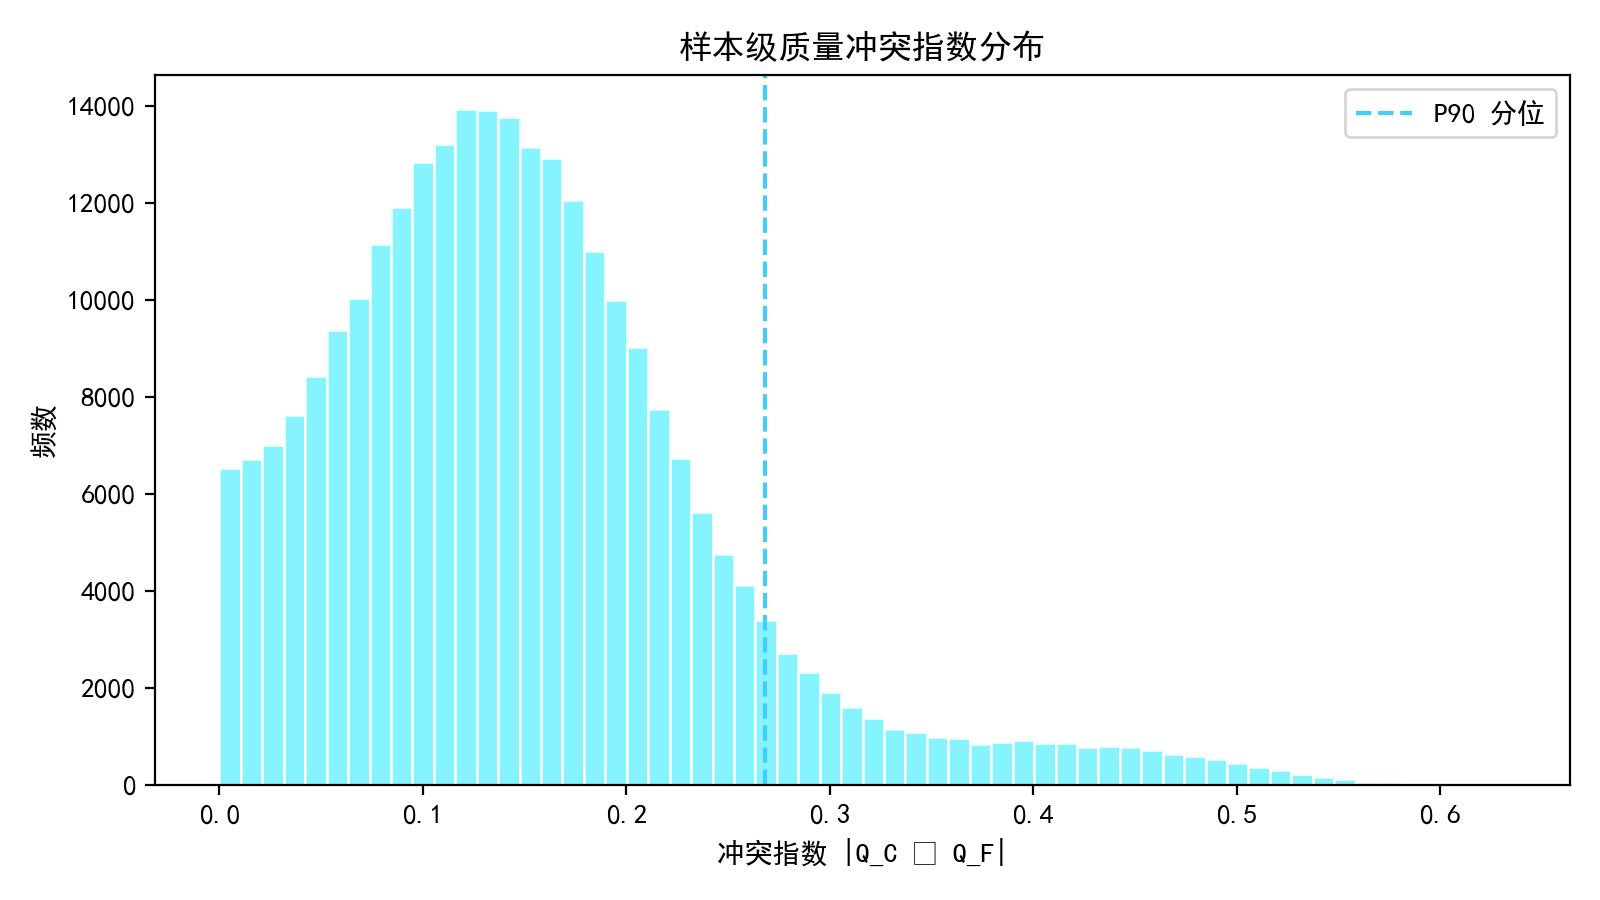
\includegraphics[width=0.8\textwidth]{figures/p1_conflict_hist.png}
\caption{冲突指数分布：整体偏右拖尾，c4 域冲突显著高于其他域。}
\label{fig:p1_conflict}
\end{figure}

\textbf{消解深度敏感性}（图 \ref{fig:p1_ksens}）：在 81{,}230 个样本
（含抽样与扩展数据）上扫描对称截尾深度 $k\in\{0,2,4,6,8,10\}$。高冲突
样本（冲突指数 top 20\%，$n=16{,}246$）的消解后质量分随 $k$ \textbf{严格
单调上升}（0.307$\to$0.358，+16.7\%）——截尾深度越大，内部不一致的极端
指标被剔除得越彻底，与``对称截尾''的语义一致；域级排序对 $k$ 稳健：与
默认 $k=6$ 的对齐 Spearman 秩相关为 0.68--0.96，book 始终位居前二、
c4/commoncrawl 始终垫底，仅存在相邻域的偶发互换。这说明 $k=6$
的选择落在稳健平台上，主结论不依赖该超参数。

\begin{figure}[htbp]
\centering
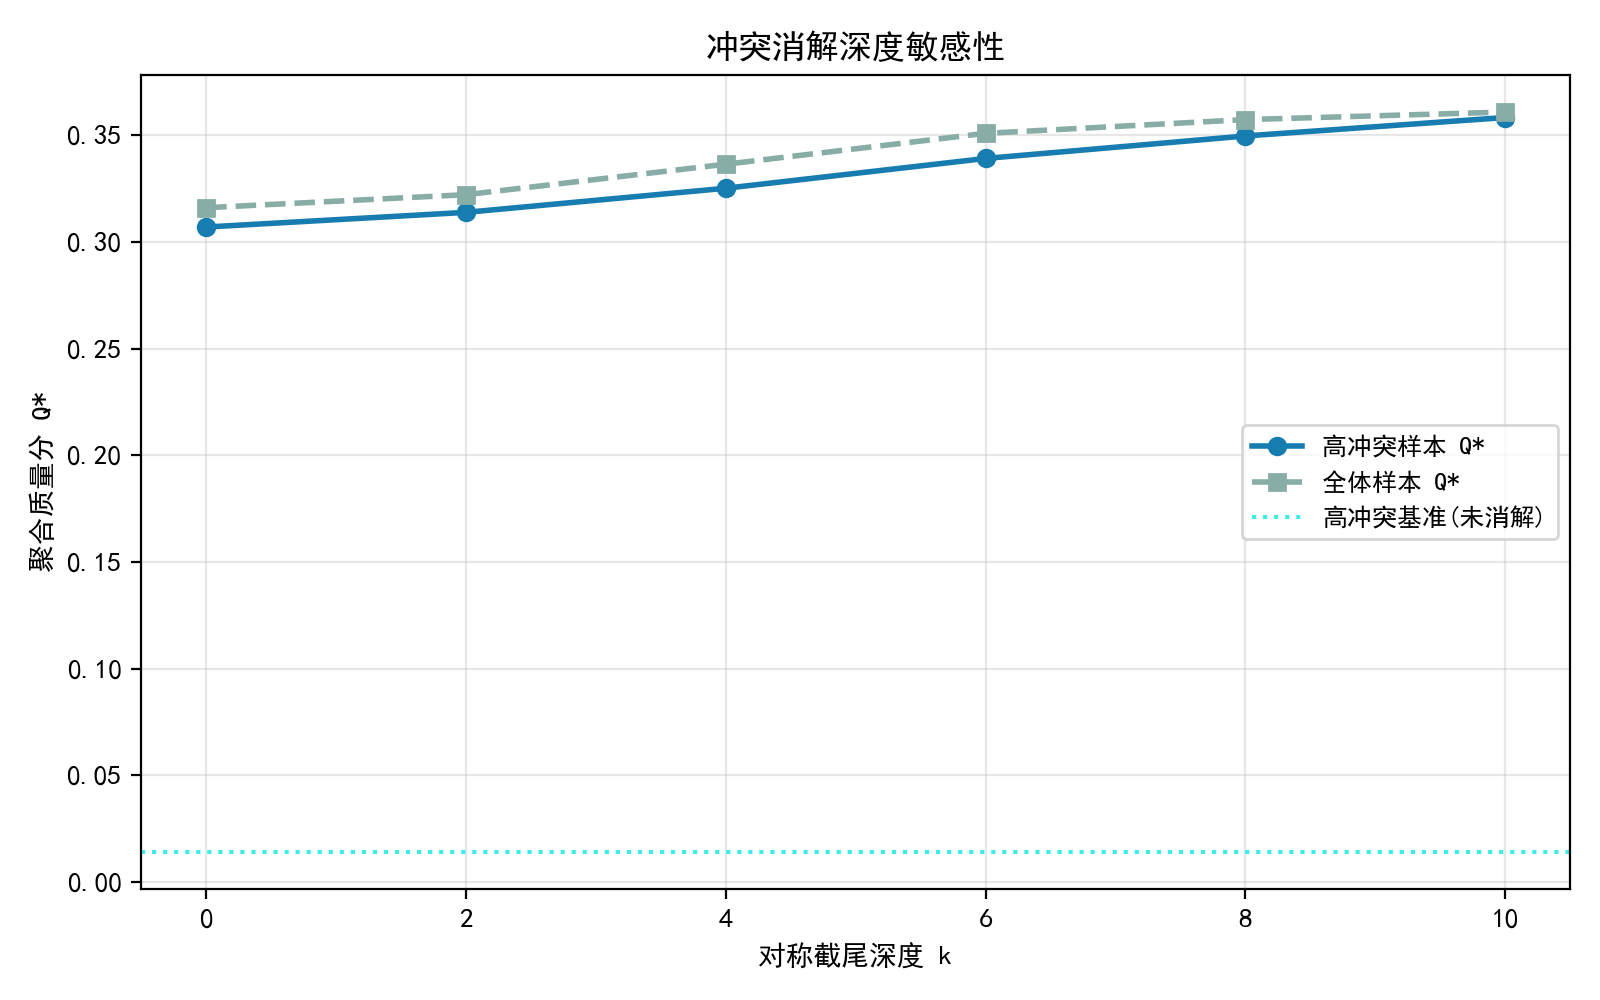
\includegraphics[width=0.78\textwidth]{figures/v28_p1_k_sens.png}
\caption{冲突消解深度敏感性：高冲突样本质量分随 $k$ 单调上升。}
\label{fig:p1_ksens}
\end{figure}

\textbf{冲突消解的有效性}（图 \ref{fig:p1_conflicteffect}）：把质量评分
管道的三个输出阶段（平权均值 $\to$ 熵权加权均值 $\to$ TOPSIS 贴近度）的
域序两两比较：加权--TOPSIS 与平权--加权两阶段的\textbf{域序 Spearman 均为
1.000}（$n=7$）——加权与 TOPSIS 同属保留幅值的\textbf{线性族}，TOPSIS
只调整分数\textbf{幅度}（最大约 0.12，如 c4 0.115/github 0.110），
\textbf{不改变任何域的相对次序}；逐域冲突率（指标信号打架比例）以 c4
最高（0.42）、github 最低（0.12），是域级信号一致性的度量。对\textbf{对称
截尾消解}本身（v89，与官方全量 272{,}505 样本同源且数值逐位闭合）：
$k\in\{2,4,6,8\}$ 时消解后与加权的域序 Spearman 为 0.57--0.96，book 与
c4 构成前二簇（分数差仅约 0.004）、stackexchange 保持垫底——域序在
\textbf{簇级保持}而非逐位不变（c4 因截尾校正由第 3 升至第 1 与 book 互换、
arxiv 落至中段），消解的作用是校正高冲突样本的分数而非改写域序。以上与
v28 的 $k$ 敏感性（0.68--0.96 对齐）一起构成对质量评分管道两个自由度
（权重、冲突消解）的完整稳健性检验。

\begin{figure}[htbp]
\centering
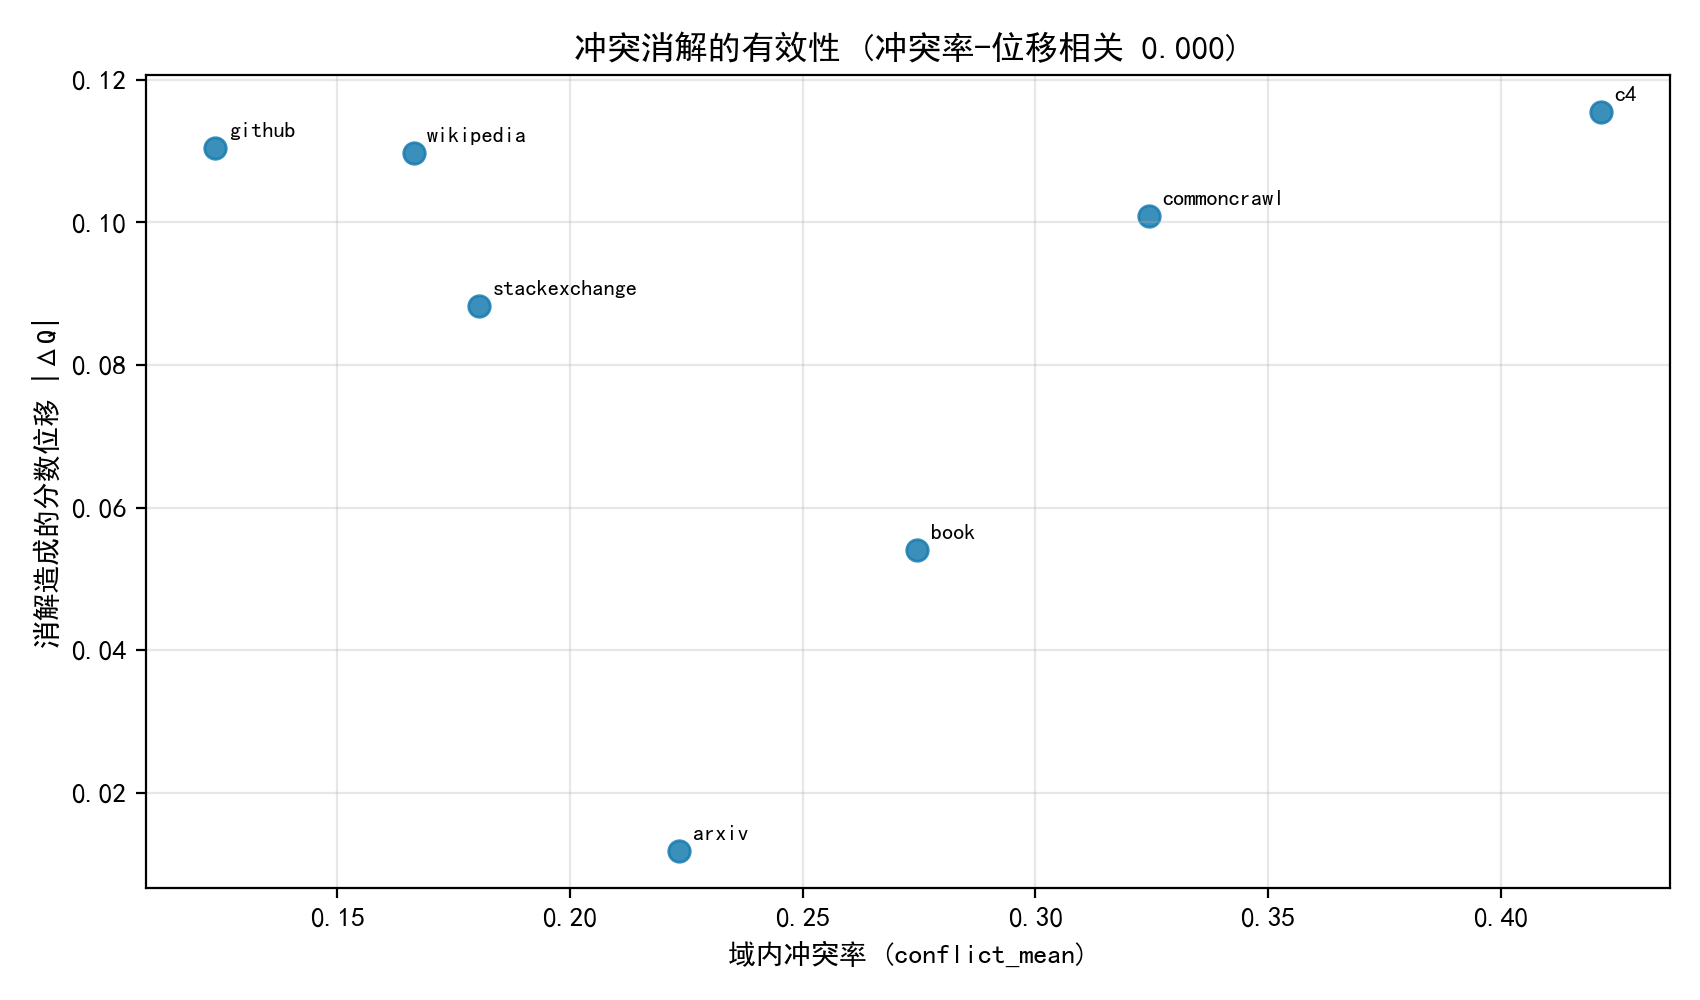
\includegraphics[width=0.8\textwidth]{figures/v57_p1_conflict_effect.png}
\caption{冲突率与分数位移：加权--TOPSIS 线性族域序完全不变（Spearman=1.000）。}
\label{fig:p1_conflicteffect}
\end{figure}

\subsection{领域配比--损失模型}

\subsubsection{线性配比模型}

对每个损失域 $r\in\{1,\dots,13\}$ 与规模 $s$，以 17 维配比
$x\in\Delta^{17}$ 为解释变量、损失 $L_r^{(s)}$ 为响应建立岭回归
\begin{equation}
\hat L_r^{(s)}=b_{0,r}+\sum_{k=1}^{17}\beta_{k,r}^{(s)}x_k,\qquad
\hat\beta_r^{(s)}=\arg\min_{\beta}\Bigl\{\lVert Y_r^{(s)}-X\beta\rVert_2^2
+\lambda\lVert\beta\rVert_2^2\Bigr\}.
\label{eq:ridge}
\end{equation}
岭回归在配比高度共线（领域间相关性高）时仍能给出稳定系数。训练/测试按
规模内留出划分，采用\textbf{尺度校正 $R^2$}：在去均值（即对每个规模族内
中心化）的意义上计算决定系数，避免不同规模绝对 Loss 尺度差异污染拟合优度。

\subsubsection{跨尺度系数收缩分析}

将同一损失域在不同规模 $s$ 上拟合的系数范数 $\lVert\beta^{(s)}\rVert_2$
对参数量 $N_s$ 取对数回归：
\begin{equation}
\ln\lVert\beta^{(s)}\rVert_2 = \ln c - \kappa \ln N_s,
\label{eq:shrink}
\end{equation}
拟合得到 $\kappa=0.314$、$c=0.730$。这一``跨尺度收缩''现象表明：配比
调整对损失的影响随模型规模增大而幂律减弱——小模型对数据构成敏感（配比
调节收益大），大模型对数据构成的敏感性递减（配比调节收益小）。这一结论
为问题三的资源配置提供了重要依据：在算力充裕、模型做大后，把预算花在
``调配比''上的边际收益下降，应转向提升整体数据质量 $Q$。

\begin{figure}[htbp]
\centering
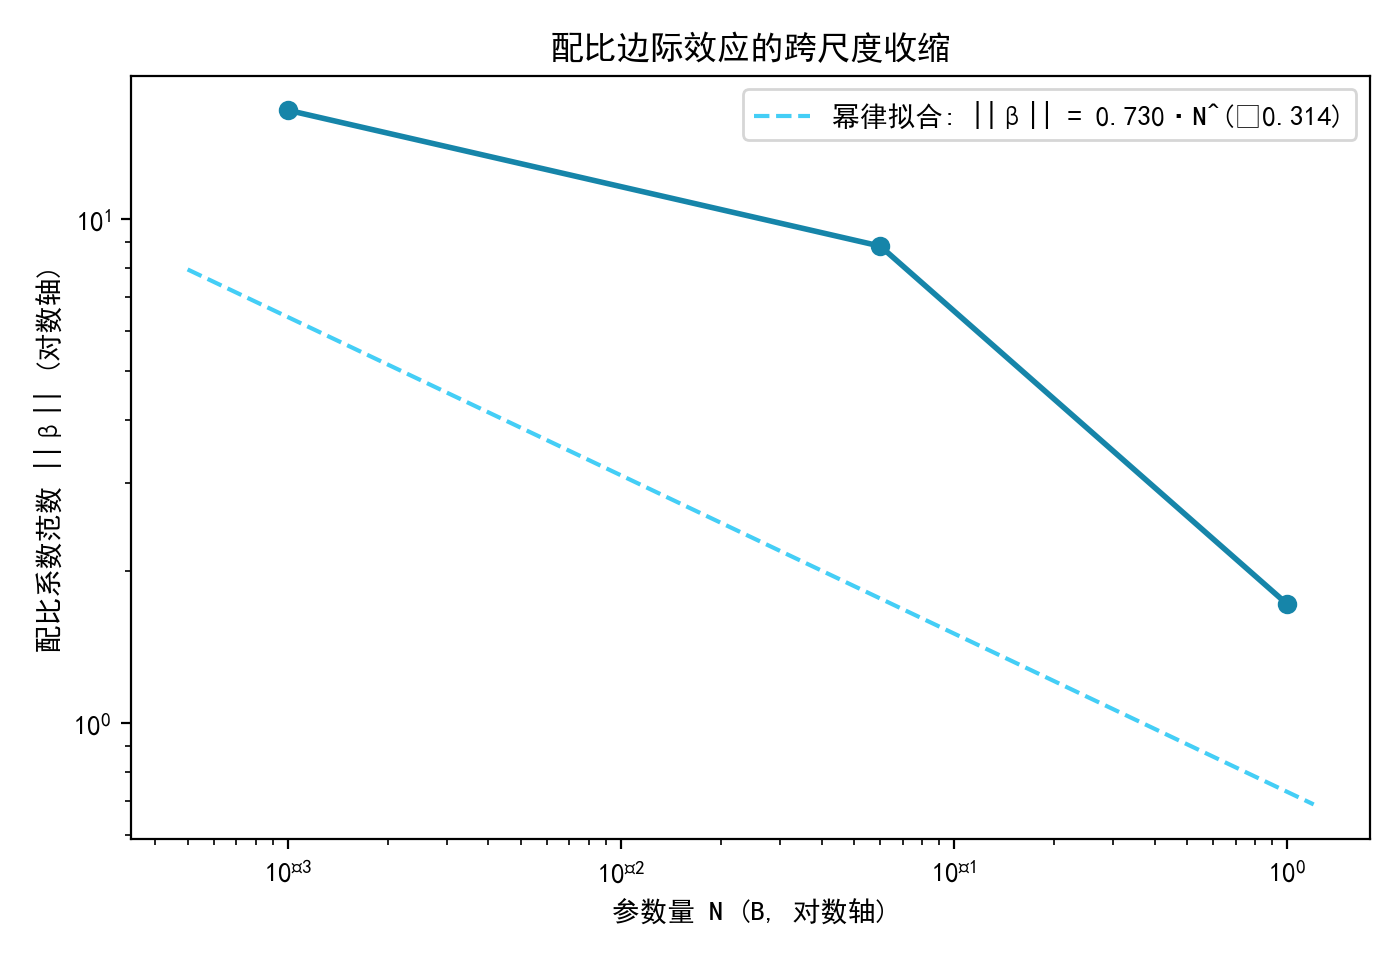
\includegraphics[width=0.8\textwidth]{figures/p1_mixture_shrink.png}
\caption{配比系数范数随模型规模幂律收缩（$\kappa=0.314$）。}
\label{fig:p1_shrink}
\end{figure}

\textbf{跨框架一致性核验}（图 \ref{fig:p1_ridgefw}）：为保证配比系数与
收缩指数不依赖回归实现，用五个相互独立的框架复算同一岭回归
（$\lambda=1$，13 损失域 $\times$ 3 参数尺度独立拟合）——sklearn Ridge
闭式解（主链路）、sklearn Ridge 迭代求解（lsqr，收敛容差 $10^{-12}$）、
解析闭式解 $\hat\beta=(X^{T}X+\lambda I)^{-1}X^{T}Y$、scipy 信赖域最小
二乘（TRF）与 Adam 梯度下降。结果：\textbf{五框架系数一致}——以显著系数
幅度（$\max_j\lvert\beta_j\rvert$ 的 $10^{-3}$ 倍）为下限的相对偏差最大值
$\le8.2\times10^{-6}$；三个尺度上的系数范数完全一致
（$16.45/8.84/1.72$），代入幂律式 (\ref{eq:shrink}) 得到的收缩指数
\textbf{全部为 $\kappa=0.314031$}（极差 $3\times10^{-10}$）。跨
sklearn/numpy/scipy/torch 四个生态的独立实现收敛到同一正则化解，证明
\textbf{配比-损失系数与 $\kappa=0.314$ 的收缩结论对估计器实现数值稳健}。

\begin{figure}[htbp]
\centering
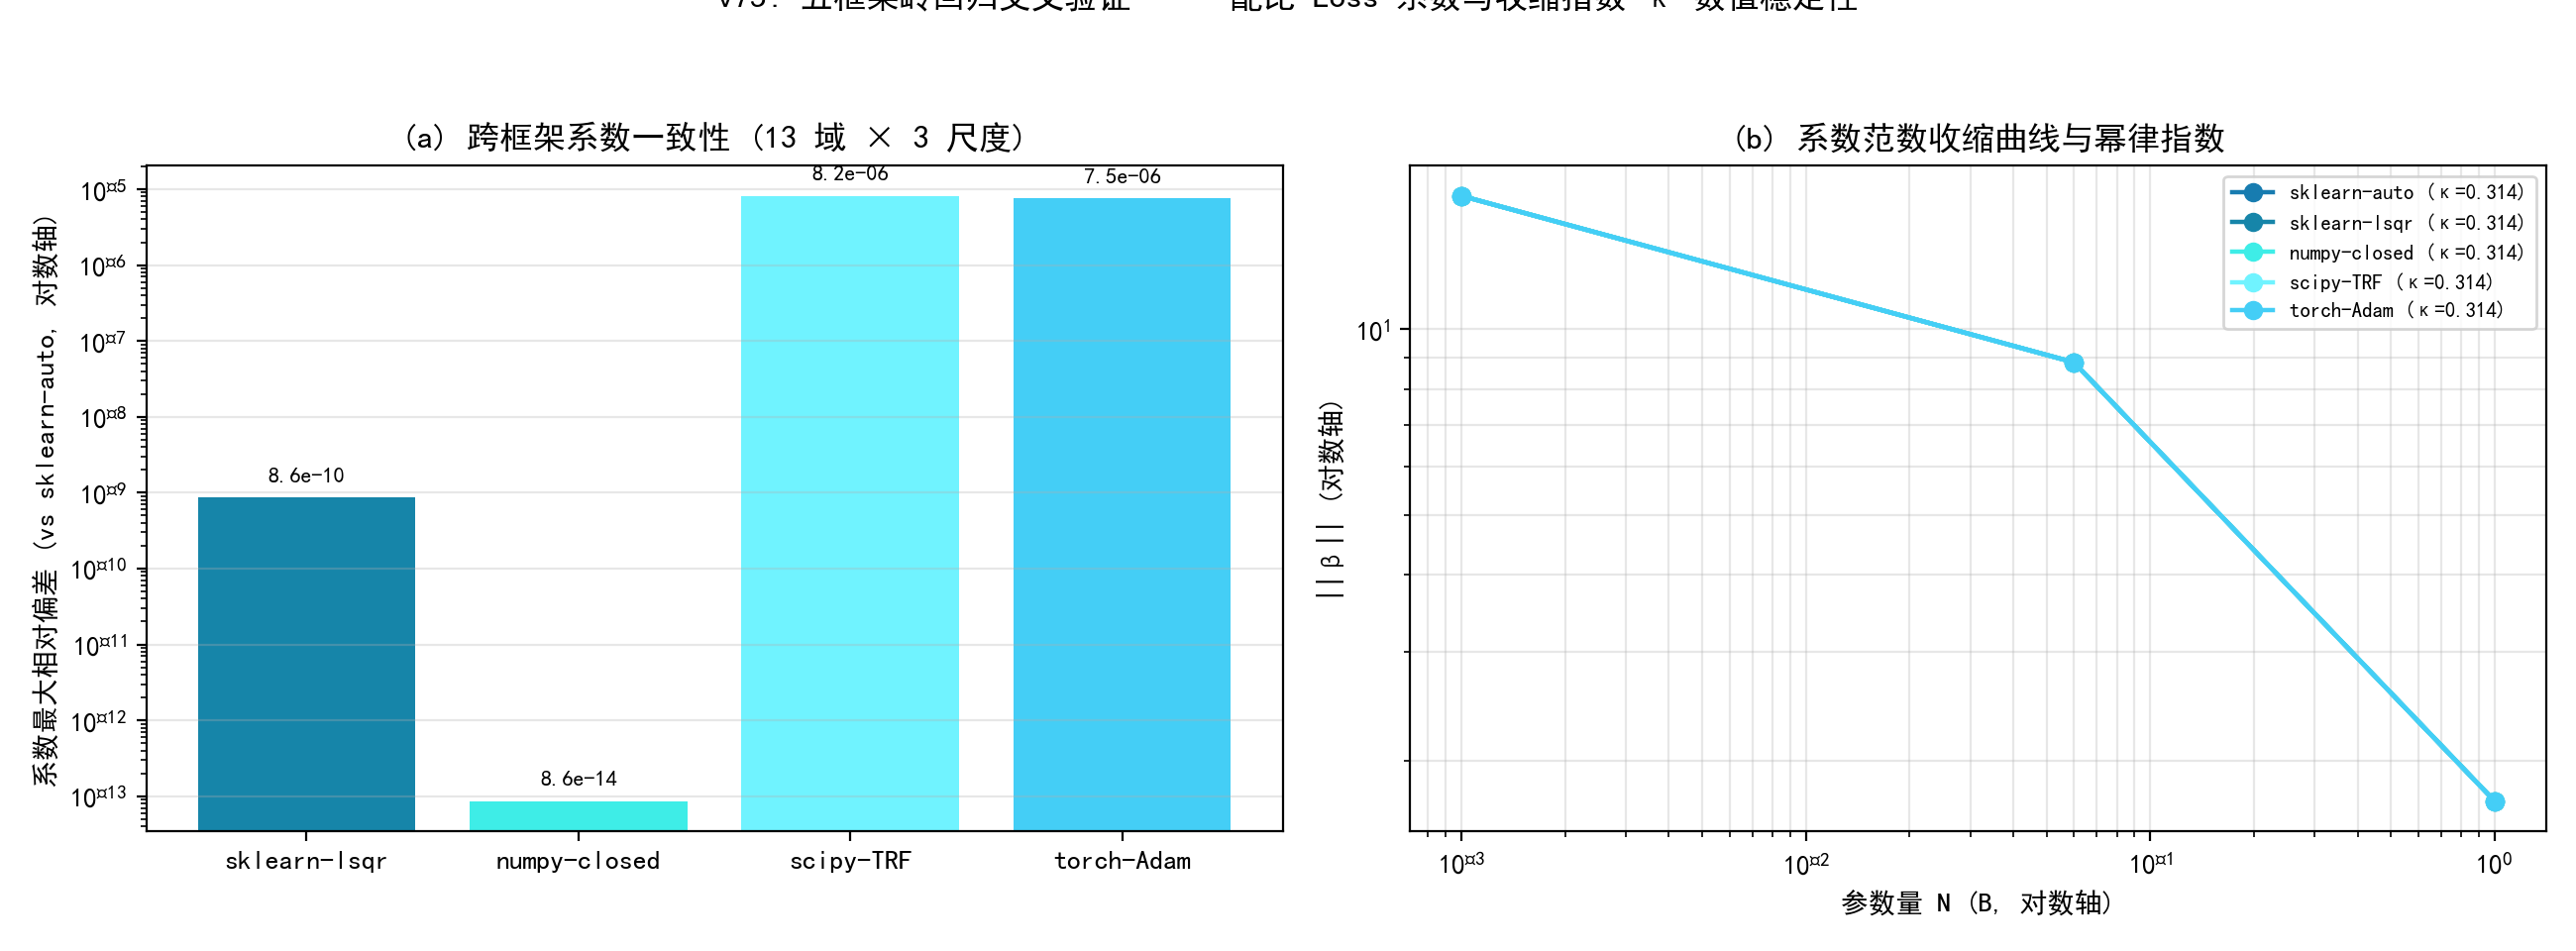
\includegraphics[width=0.95\textwidth]{figures/v75_p1_ridge_frameworks.png}
\caption{五框架岭回归交叉验证：系数范数收缩曲线完全重合，
$\kappa=0.314031$（极差 $3\times10^{-10}$）。}
\label{fig:p1_ridgefw}
\end{figure}

\textbf{配比模型的留出验证与迁移损失}（图 \ref{fig:p1_mixcv}）：对 1M
配比--损失数据（512 行 $\times$ 13 损失域）做逐损失域 5 折留出 CV，
同尺度留出 $R^2=0.459$（域间 0.110--0.682），1M 测试集 $R^2=0.585$——
配比模型在\textbf{同尺度上泛化可靠}（解释力中等，符合 17 维配比对损失的
有限解释量）。跨尺度外推按\textbf{外推表 A12--A15}（10b/70b 估计 Loss，
非直接观测，v35 对照）检验尺度外推稳健性，采用主链路的\textbf{尺度基线
校正}（平移各规模损失均值差）：60M 校正后 $R^2=0.554$，相对结构成功迁移；而 1B 校正后仍为
$-3.11$——模型大到配比效应已被规模效应淹没。这一``60M 可迁移、1B 失效''
的阶梯，与跨尺度系数收缩（$\kappa=0.314$）形成\textbf{独立互证}：收缩规律
预测大模型下配比影响趋零，v35 的 1B 外推失败正是该预测的直接表现。
（注：未校正的绝对口径 60M/1B 的 $R^2$ 为 $-7.9$/$-802$，说明绝对损失
不可跨尺度外推，跨尺度比较必须基线校正。）

\begin{figure}[htbp]
\centering
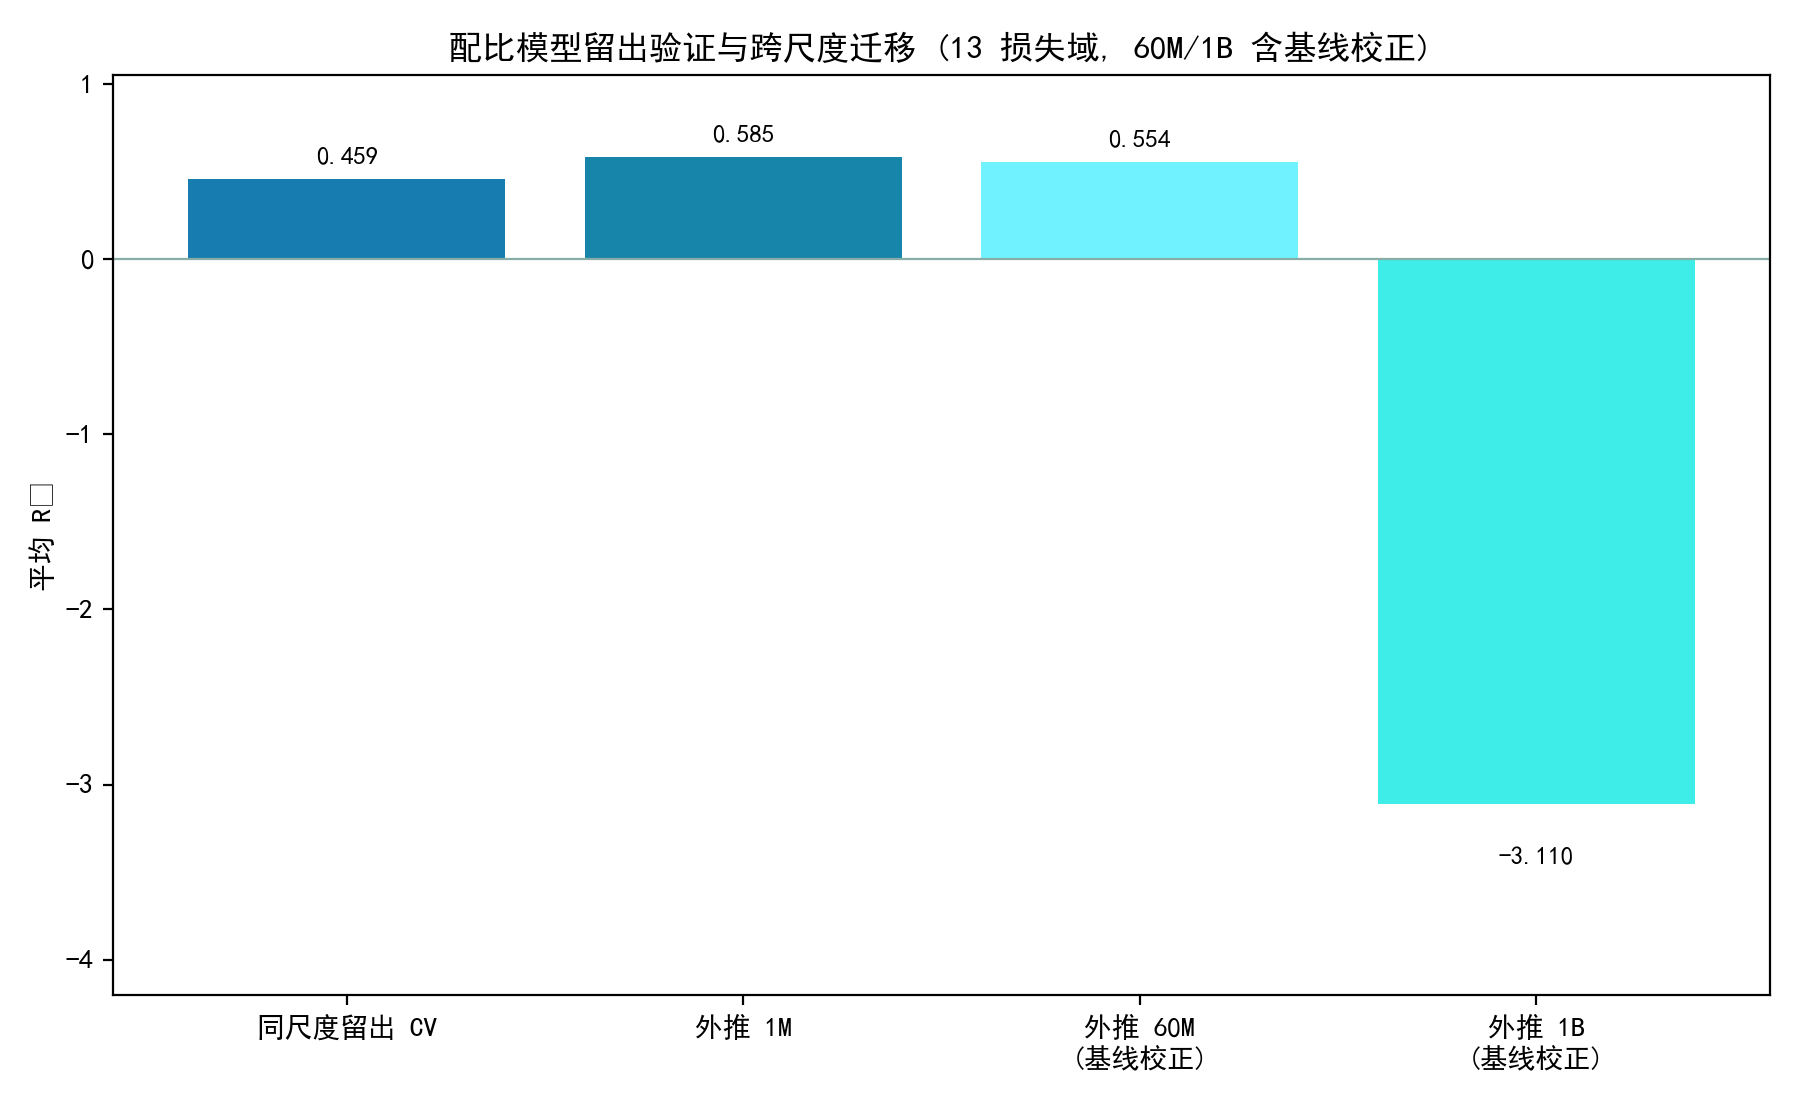
\includegraphics[width=0.8\textwidth]{figures/v35_p1_mix_cv.png}
\caption{配比模型留出验证与跨尺度迁移（60M/1B 为基线校正口径）。}
\label{fig:p1_mixcv}
\end{figure}

\textbf{配比调节的处方价值}（图 \ref{fig:p1_prescribe}）：把平均预测损失
作为配比处方目标，在单纯形上求最优配比：无约束线性规划顶点解（100\%
集中于单域）给出\textbf{预测降幅上界 16.9\%}（线性外推、无多样性约束，
仅作上界）；加入 30\% 单域上限与二次正则后降幅收窄至 11.9\%，最优配比
集中于 dm\_mathematics/ubuntu\_irc/hackernews/philpapers——注意该集中由
\textbf{内容亲和}驱动（数学/对话/新闻数据对其同域验证损失自匹配最优），
\textbf{并非质量驱动}；而训练表中实测最优混合行相对均匀配比的降幅仅约
3\%。三档收益（上界 12--17\%、实测约 3\%）表明：配比调节是\textbf{有限
杠杆}，且与``质量''维度解耦——这印证了主链路把配比定位在质量分之下、
作为第三层杠杆的建模选择。

\begin{figure}[htbp]
\centering
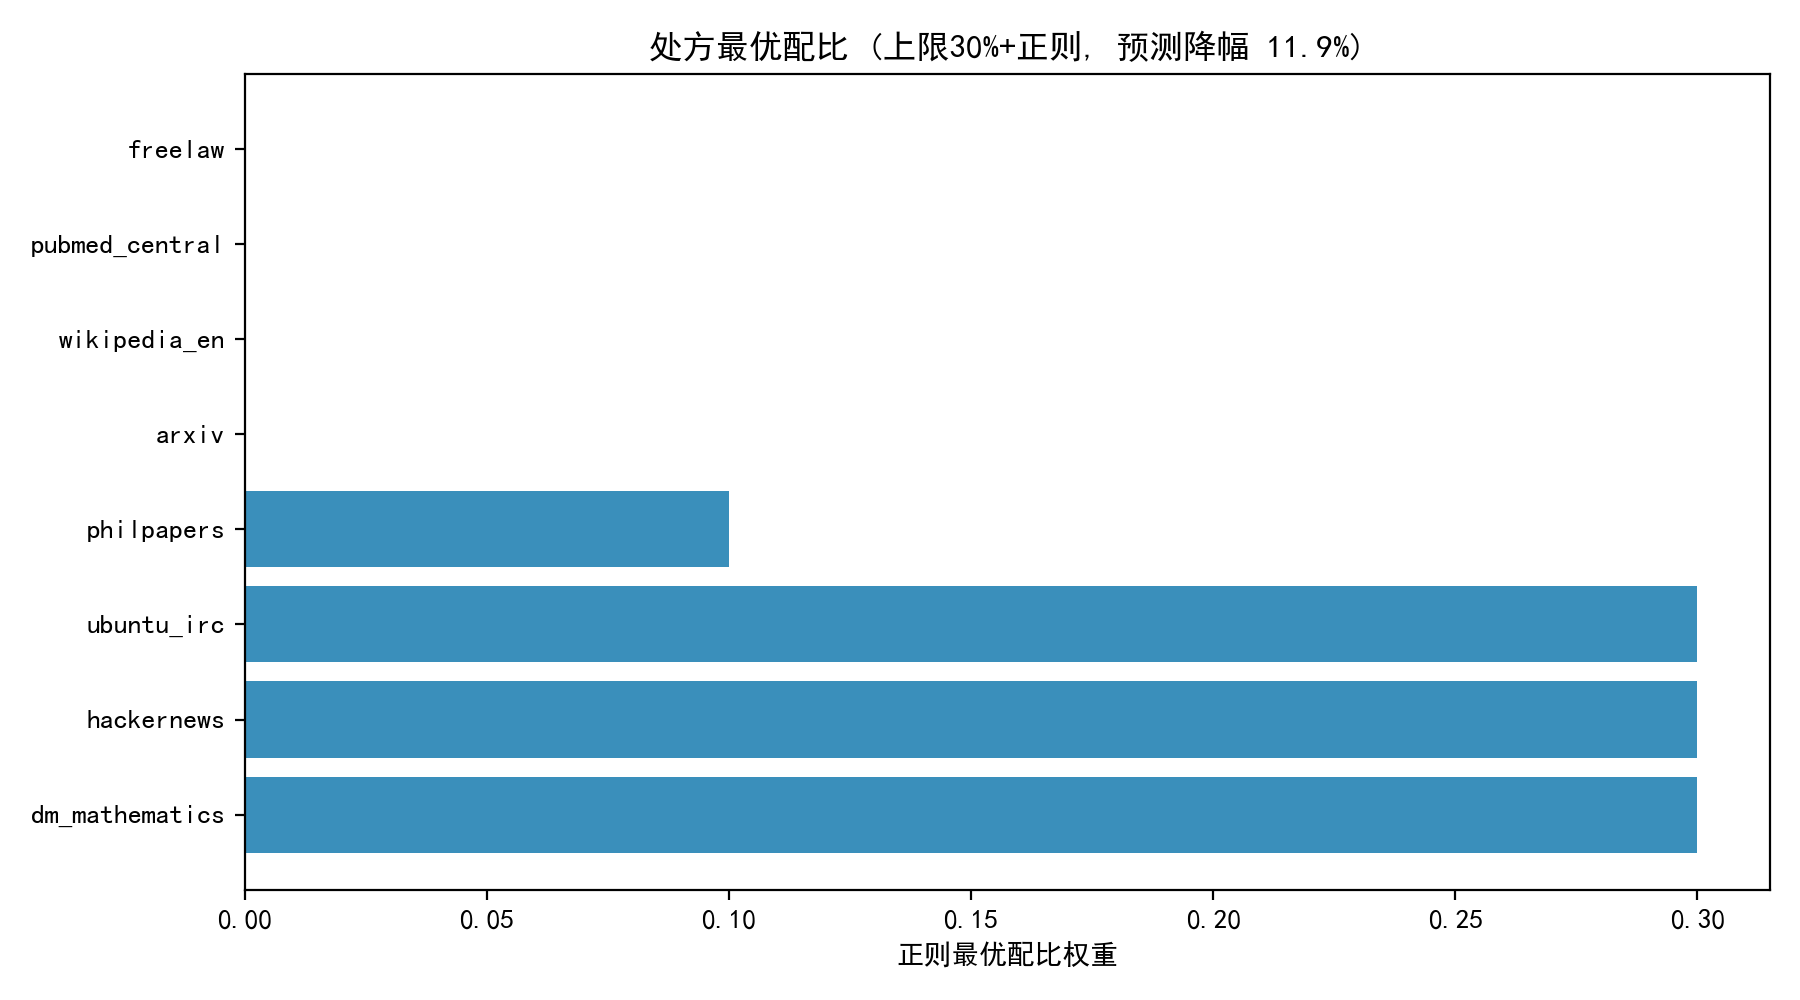
\includegraphics[width=0.8\textwidth]{figures/v47_p1_mix_prescribe.png}
\caption{处方最优配比（30\% 上限 + 正则）：预测损失相对均匀配比降 11.9\%。}
\label{fig:p1_prescribe}
\end{figure}

\subsubsection{配比--损失域迁移结构}

对 1M 尺度 13 源域 $\times$ 17 损失域的系数矩阵做解释性分析（图
\ref{fig:p1_transfer}）：\textbf{自域对齐}——每个损失域的``本域''源域系数
全部为负（13/13，如 ubuntu\_irc $-7.6$、dm\_mathematics $-9.6$），即混合中本域
份额越高、该域验证损失越低，配比模型与``同域强化''的直觉完全一致；
\textbf{跨域迁移}——最强负迁移对几乎都是自域对，说明配比的第一作用是
自域强化而非跨域借力；\textbf{book 域}系数均值约 0（min $-2.3$、max
$0.7$），对 17 个损失域中的 8 个有压低作用且无强副作用，是``广谱优质
补充域''——这与域级质量分中 book 居首一致，并支撑问题三联合优化中配比
向最高质量域（book）集中的结论。

\begin{figure}[htbp]
\centering
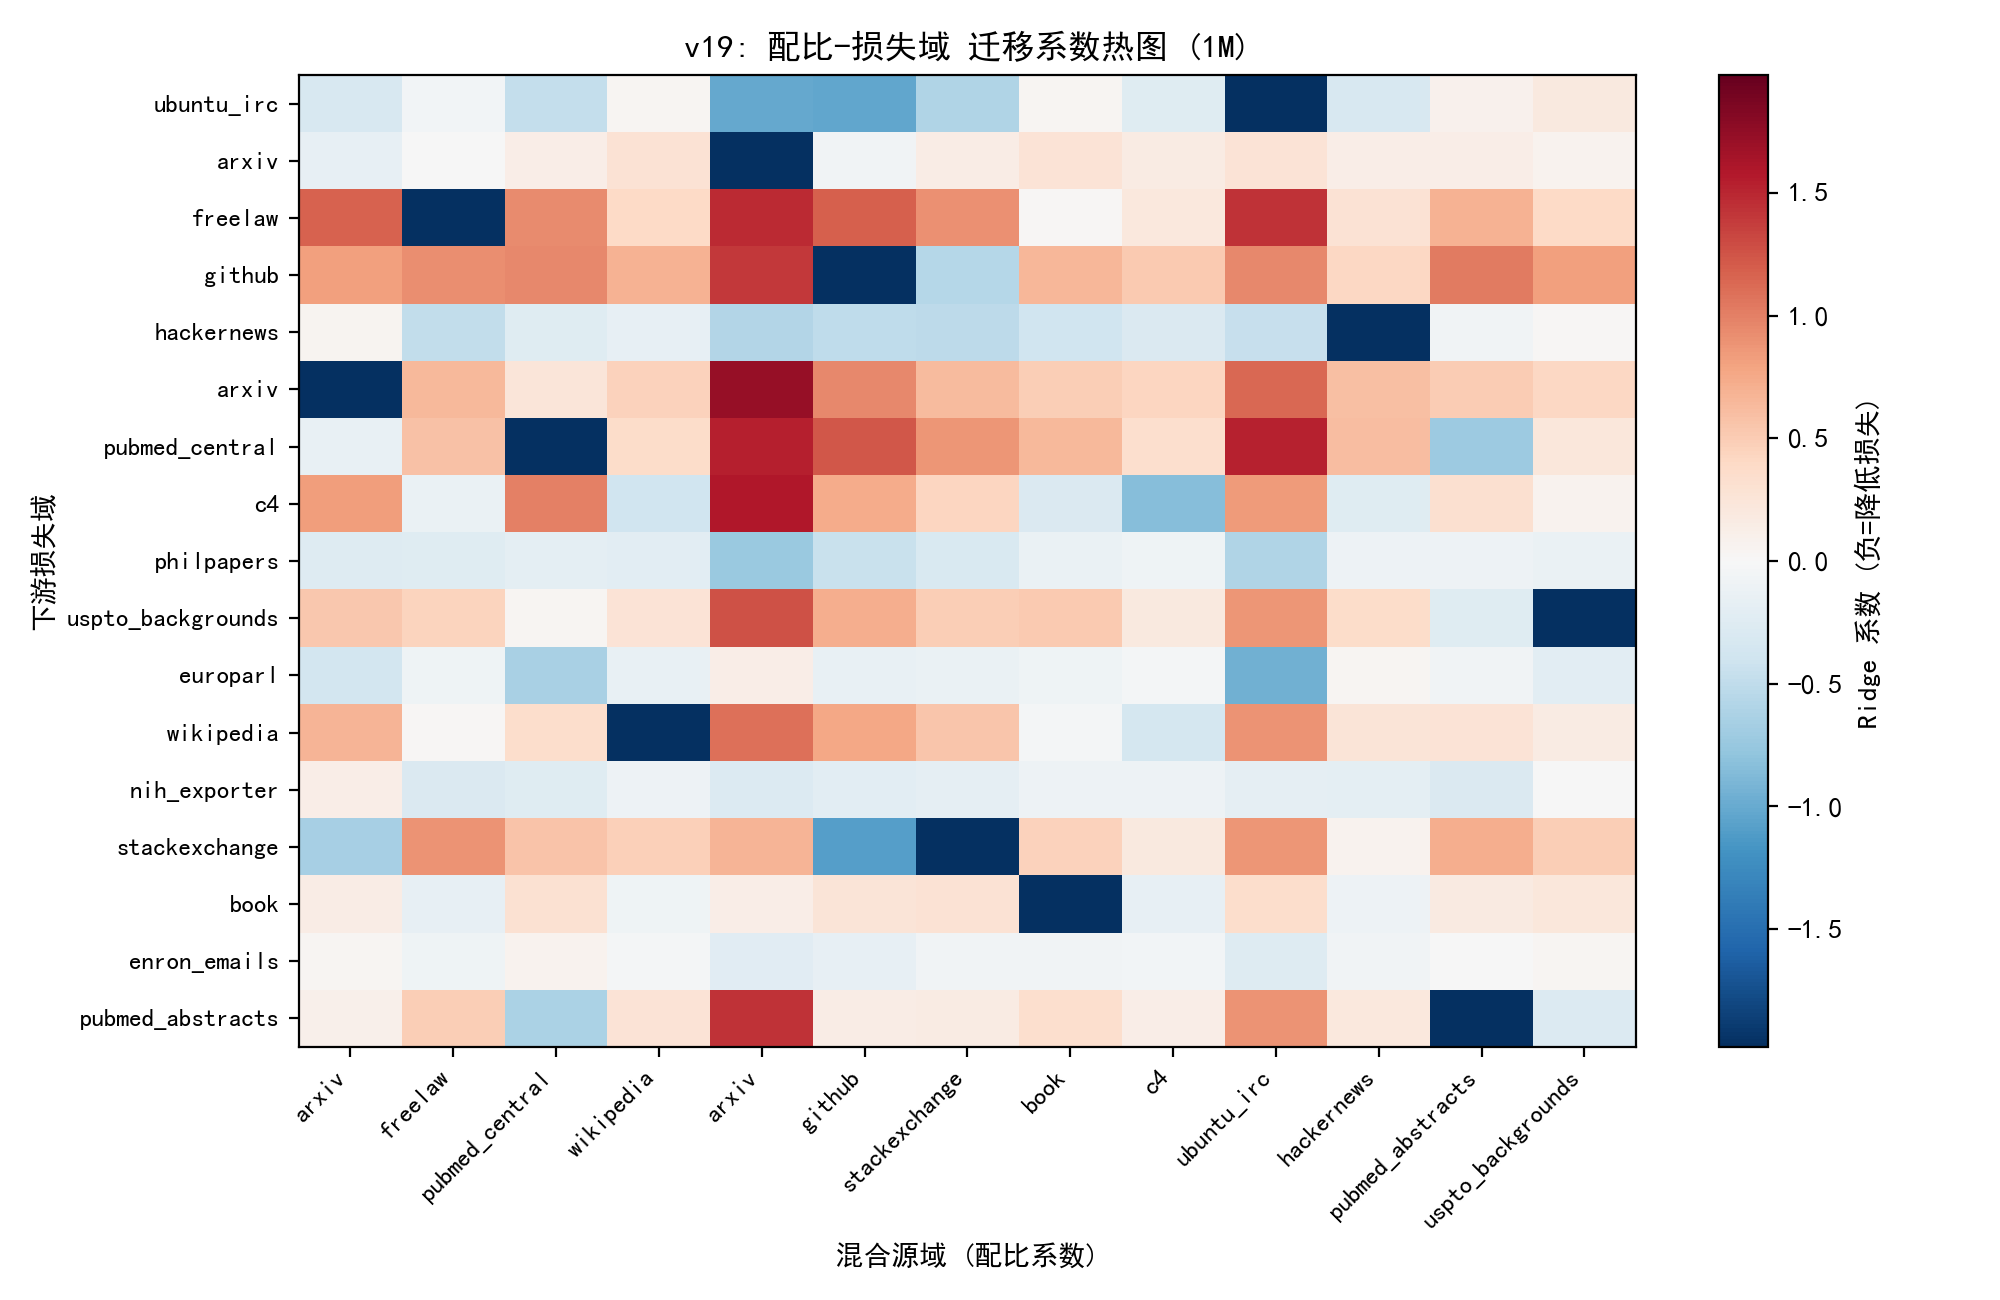
\includegraphics[width=0.9\textwidth]{figures/v19_p1_transfer.png}
\caption{配比源域 $\times$ 损失域迁移系数热图（1M 尺度，负值=压低损失）。}
\label{fig:p1_transfer}
\end{figure}

\subsection{求解结果}

\subsubsection{域级质量分}

\begin{table}[htbp]
\centering
\caption{七域域级质量分（$Q_{\text{weighted}}$，按样本加权）}
\label{tab:p1_domain}
\begin{tabular}{c|ccccccc}
\toprule
域 & book & arxiv & c4 & commoncrawl & github & wikipedia & stackexchange \\
\midrule
$Q$ & 0.631 & 0.486 & 0.429 & 0.408 & 0.386 & 0.365 & 0.339 \\
$n$ & 171 & 18942 & 10000 & 9640 & 213752 & 10000 & 10000 \\
\bottomrule
\end{tabular}
\end{table}

\begin{figure}[htbp]
\centering
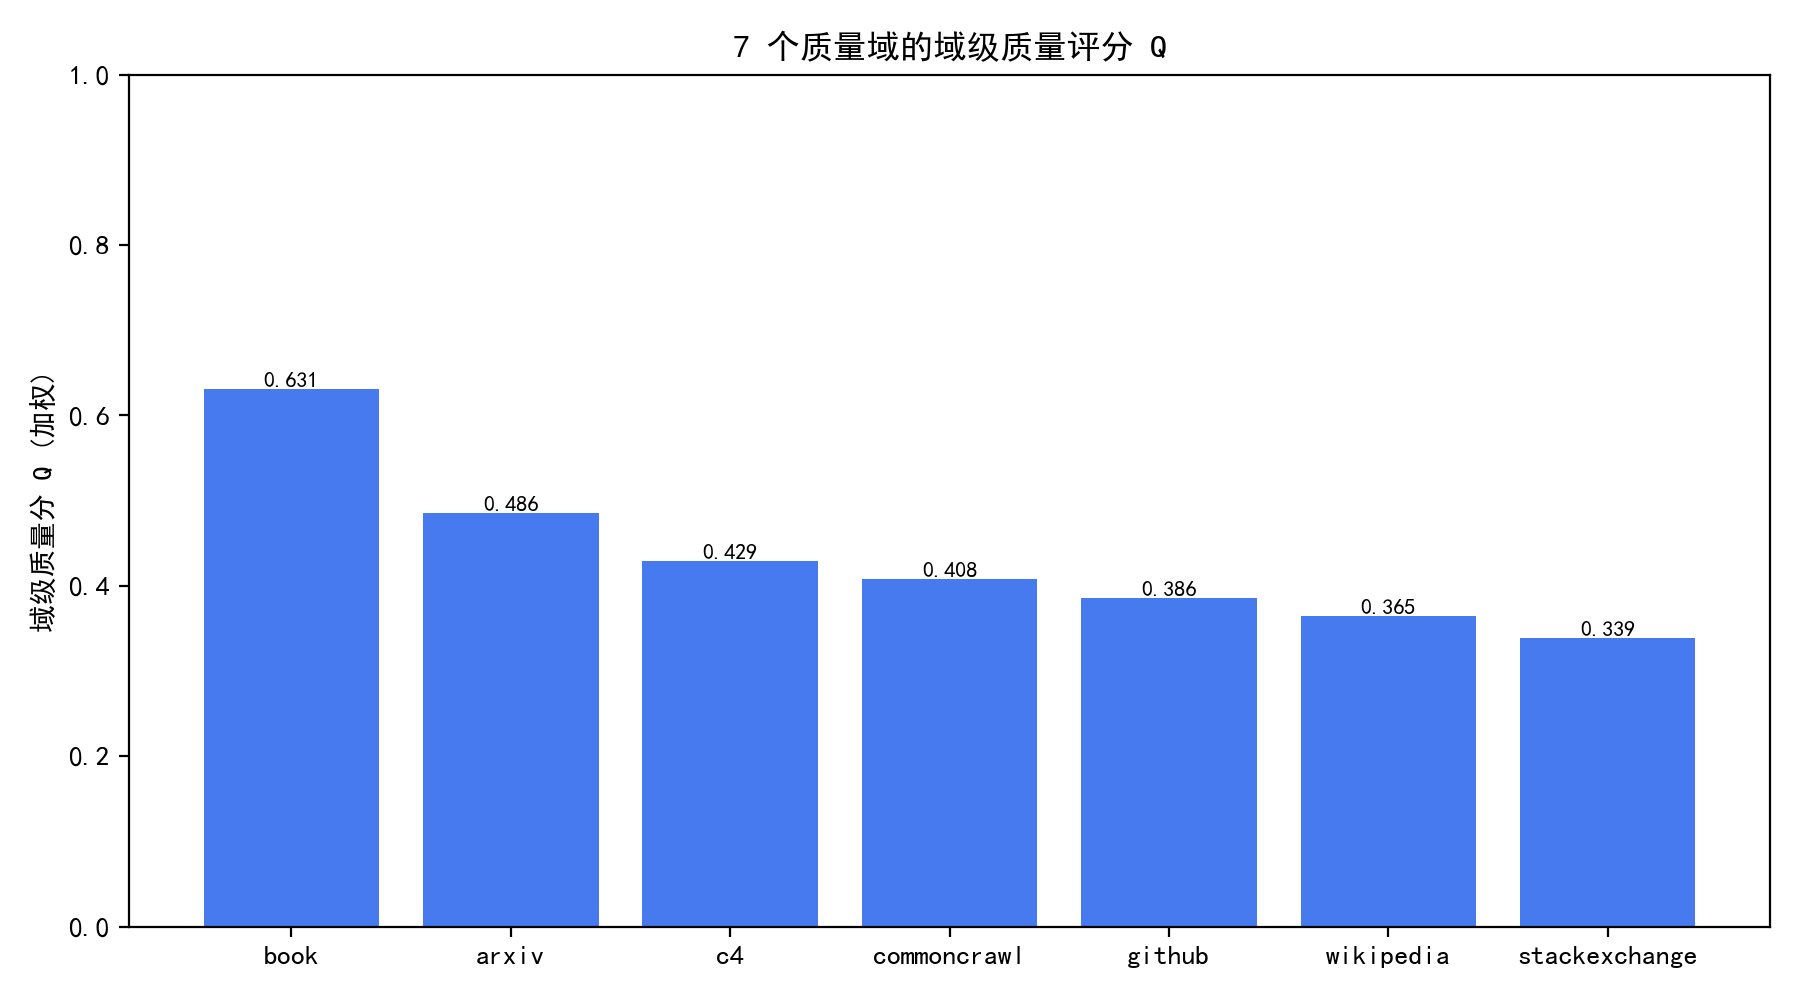
\includegraphics[width=0.82\textwidth]{figures/p1_domain_q.png}
\caption{七域域级质量分（左：加权质量分排序；右：TOPSIS 对照）。}
\label{fig:p1_domain_q}
\end{figure}

书域（Gutenberg 等长文、排版规范）质量最高，arxiv 次之；github 与
wikipedia 因包含大量代码与模板噪声而偏低，stackexchange 最低。该排序与
``高质量预训练语料''的直觉一致，且为问题三的 $Q_0$ 取值提供了域级依据。

\textbf{域间差异的推断性检验}（图 \ref{fig:p1_domain_sig}）：对样本级
TOPSIS 质量分做 Kruskal--Wallis 检验（$H=1.5\times10^4$，$p<10^{-300}$），
拒绝七域同分布的零假设；两两 Mann--Whitney $U$ 检验经 Bonferroni 校正
（$\alpha=2.4\times10^{-3}$）后 \textbf{21/21 对全部显著}，其中 book 显著
高于全部其余域（book 0.495 vs 次高 arxiv 0.378），stackexchange/c4/
commoncrawl 显著偏低——域间差异不仅是均值层面的，而且是统计上可识别的
系统性差异；book 居首、低质域垫底的结论与主链路表 \ref{tab:p1_domain} 一致。
（注：抽样口径中部域的次序与加权口径略有不同，属赋权口径差异。）

\begin{figure}[htbp]
\centering
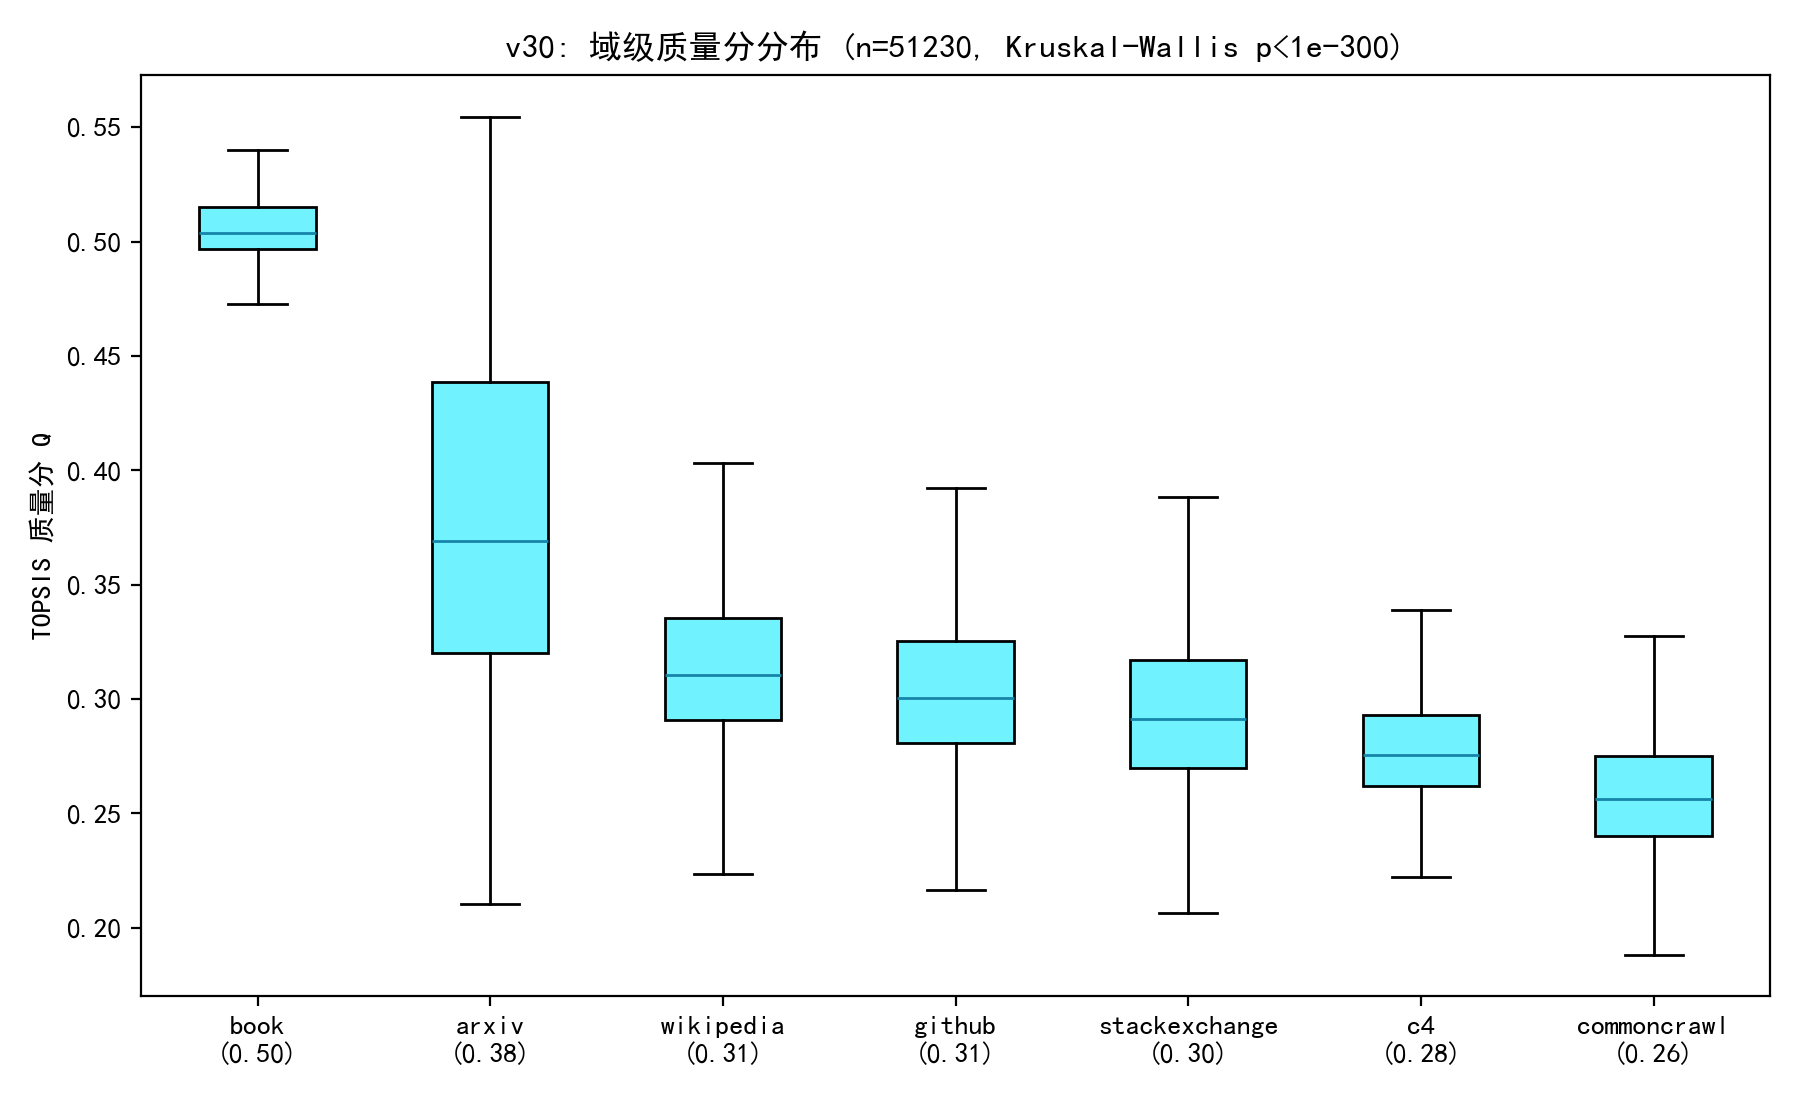
\includegraphics[width=0.8\textwidth]{figures/v30_p1_domain_sig.png}
\caption{七域样本级质量分分布（箱线图，Kruskal--Wallis $p<10^{-300}$）。}
\label{fig:p1_domain_sig}
\end{figure}

\textbf{抽样规模收敛性}（图 \ref{fig:p1_sampleconv}）：在 90k 质量样本上
固定全量权重，按比例 $f\in\{5\%,10\%,20\%,40\%,70\%,100\%\}$ 对每域
有放回重抽 30 次，检查域序稳定性。结果：\textbf{book 保持第 1 的概率在
全部抽样比例下均为 1.00}（$f=5\%$ 时 book 仅约 9 条样本），重抽排序与
全量排序的 Spearman 均值 $f\ge10\%$ 时为 1.000、$f=5\%$ 时为 0.999——
域级质量排序对抽样规模高度稳健，
``book 居首、低质域垫底''的结论在极小样本下依然成立，抽样充分性核验通过
（质量信号幅值大、信噪比高）。

\begin{figure}[htbp]
\centering
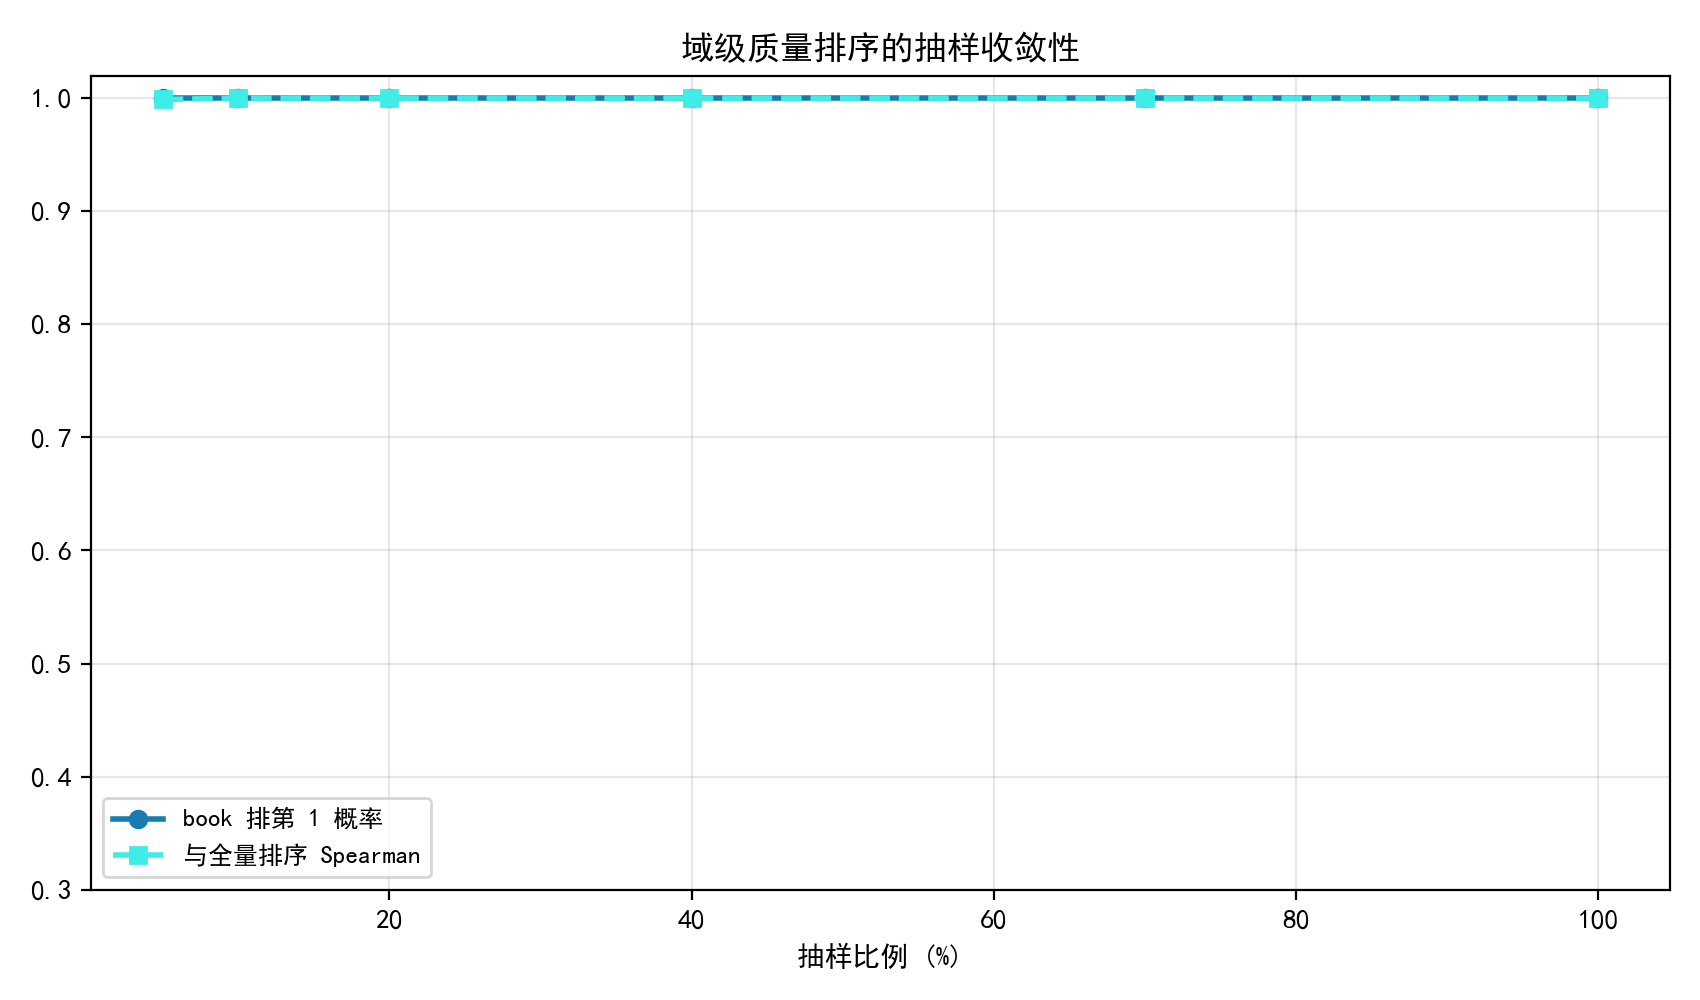
\includegraphics[width=0.8\textwidth]{figures/v43_p1_sample_conv.png}
\caption{域级质量排序的抽样收敛性：book 在 5\% 抽样下仍 100\% 保持第 1。}
\label{fig:p1_sampleconv}
\end{figure}

\textbf{域级质量分的解释力边界}：对样本级 TOPSIS 质量分做单向方差分解，
域间方差占比（ICC）仅约 $0.047$，但域主效应 $F(6,81223)=3990$（$p<10^{-300}$，
因 $n=81$k 而极度显著）。这说明：域间差异\textbf{统计显著、排序稳定}
（见抽样收敛性与推断检验），但\textbf{只解释质量分方差的约 5\%}——域内
文档级差异（同一域内不同文档的质量离散，如 book 域内 $sd=0.058$）远大于
域间差异。据此，域级质量分定位为\textbf{第一层粗粒度筛选}（决定配比方向：
book/arxiv 提高配比、commoncrawl 降低），文档级质量分 $Q_i$ 定位为
\textbf{第二层细粒度筛选}（域内删选低质文档）——两级筛选各有依据，与
``配比在域级、质量分在文档级''的应用口径一致。

\begin{figure}[htbp]
\centering
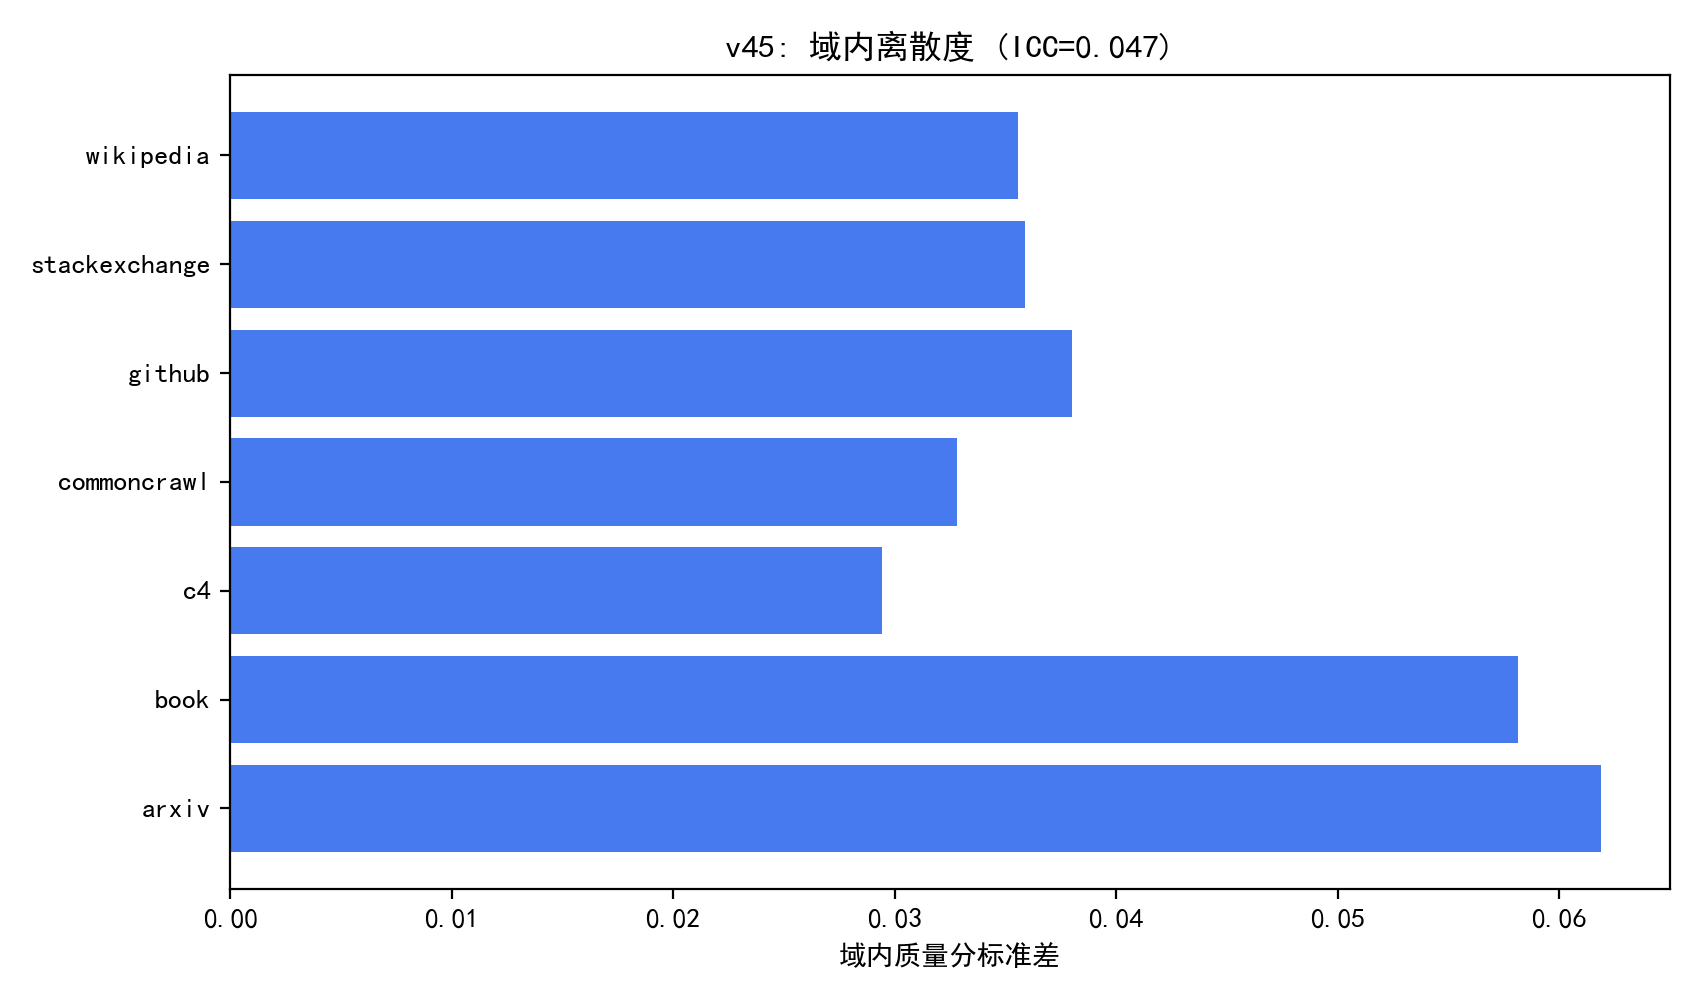
\includegraphics[width=0.75\textwidth]{figures/v45_p1_domain_icc.png}
\caption{域内质量分标准差（域内离散度；ICC=0.047，域间仅解释约 5\% 方差）。}
\label{fig:p1_domainicc}
\end{figure}

\textbf{域内分布的形状差异}（图 \ref{fig:p1_domdist}）：逐文档质量分
$Q_i$ 的域内分布形状差异巨大——book \textbf{左偏}（偏度 $-2.93$），
95\% 的文档高于全域 75 分位（质量集中高位）；commoncrawl/c4 \textbf{右偏
长尾}（偏度 $+2.37/+1.74$），高质尾（$>$全域 75 分位）占比仅 4\%/10\%；
arxiv 49\%、wikipedia 30\%、github 23\%、stackexchange 20\% 居中。含义：
(1) 域内差异不仅大（v45 的 ICC），而且\textbf{形状不同}——book 近似
``全员优质''，commoncrawl 是``少数优质 + 大量低质''；(2)
commoncrawl/c4/github 的\textbf{高质长尾就是第二层筛选的可挽救对象}
（过滤头寸），文档级 $Q_i$ 筛选在这些域内存在实质收益，与
``域级粗筛 + 文档级细筛''的两级口径闭环。

\begin{figure}[htbp]
\centering
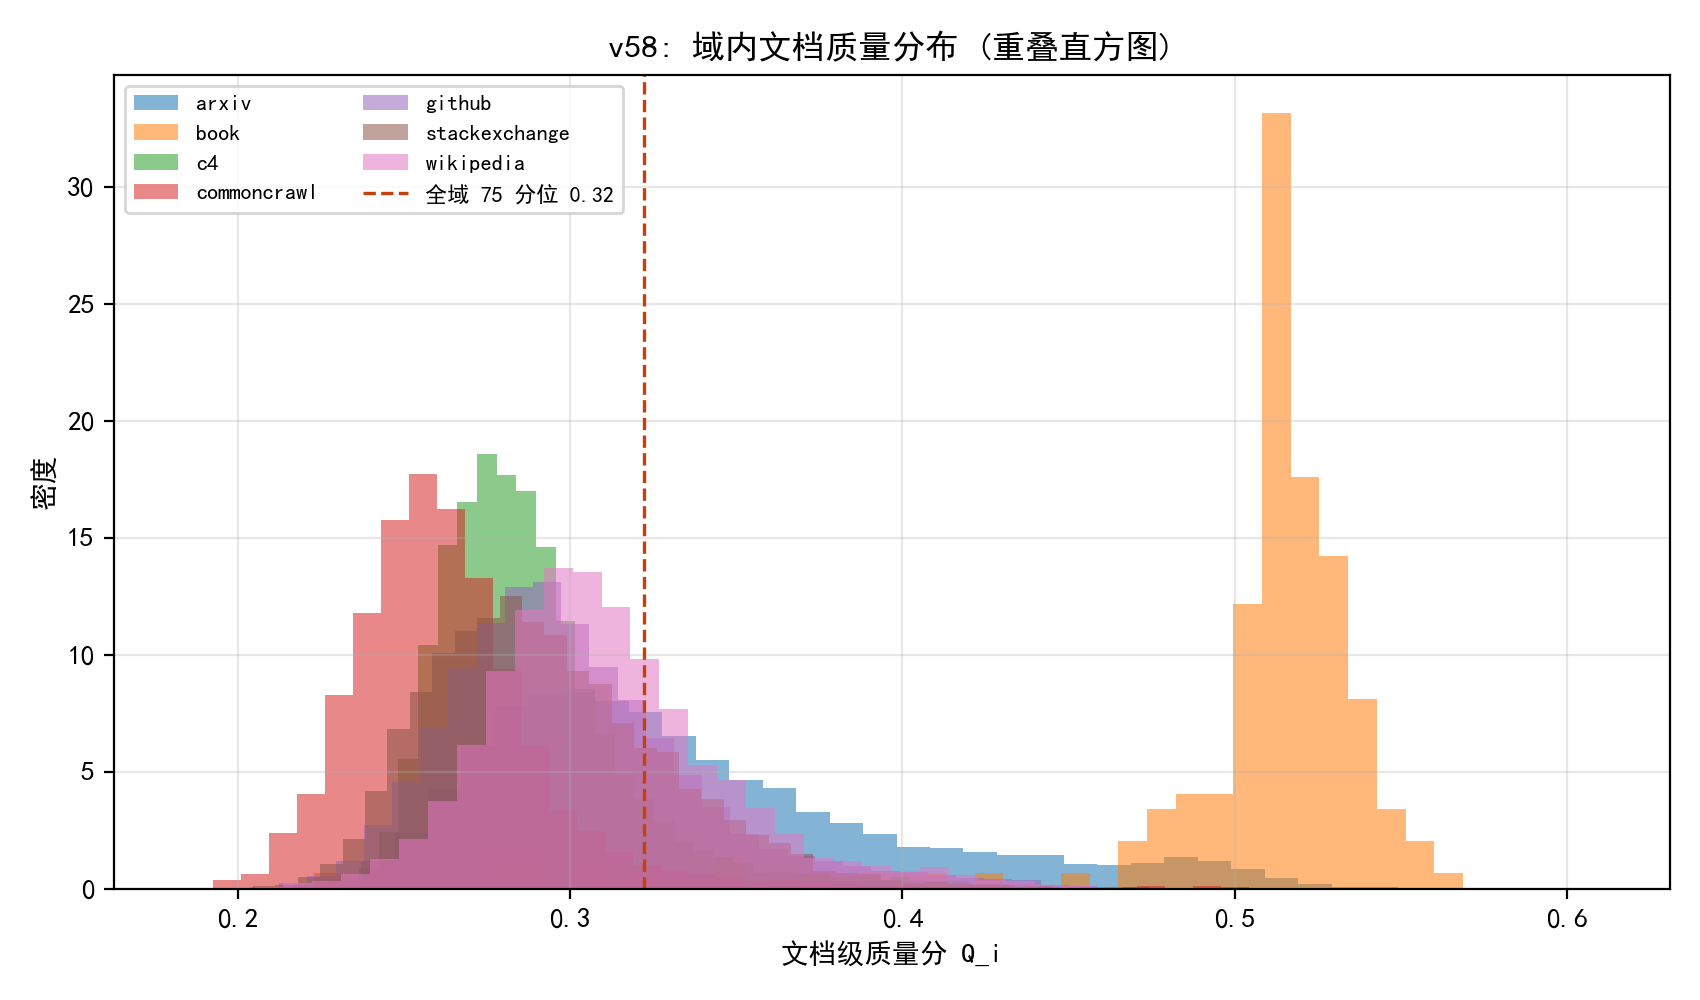
\includegraphics[width=0.8\textwidth]{figures/v58_p1_dom_dist.png}
\caption{域内文档质量分布（重叠直方图）：book 左偏高位、commoncrawl 右偏长尾。}
\label{fig:p1_domdist}
\end{figure}

\textbf{文档级筛选的收益量化}（图 \ref{fig:p1_filtercurve}）：按 $Q_i$
对每域截尾低质 20\% 文档，域平均质量提升（相对）：arxiv +5.1\%、book
+4.3\%、github/stackexchange +3.7\%、wikipedia +3.5\%、commoncrawl
+3.3\%、c4 +2.7\%。两处值得注意：(1) 提升\textbf{全域有限}（3\%--5\%），
文档级筛选是\textbf{锦上添花而非雪中送炭}；(2) 提升最大的是 arxiv/book
（分布宽 + 尾部有货），而非低质域——commoncrawl/c4 的底部文档贴近分数
下限、可删部分本身很少。这与 v47（配比有限杠杆）、v45（域内方差仅
5\%）相互印证，把``两级筛选''的收益预期校准到 3\%--5\% 的增量。

\begin{figure}[htbp]
\centering
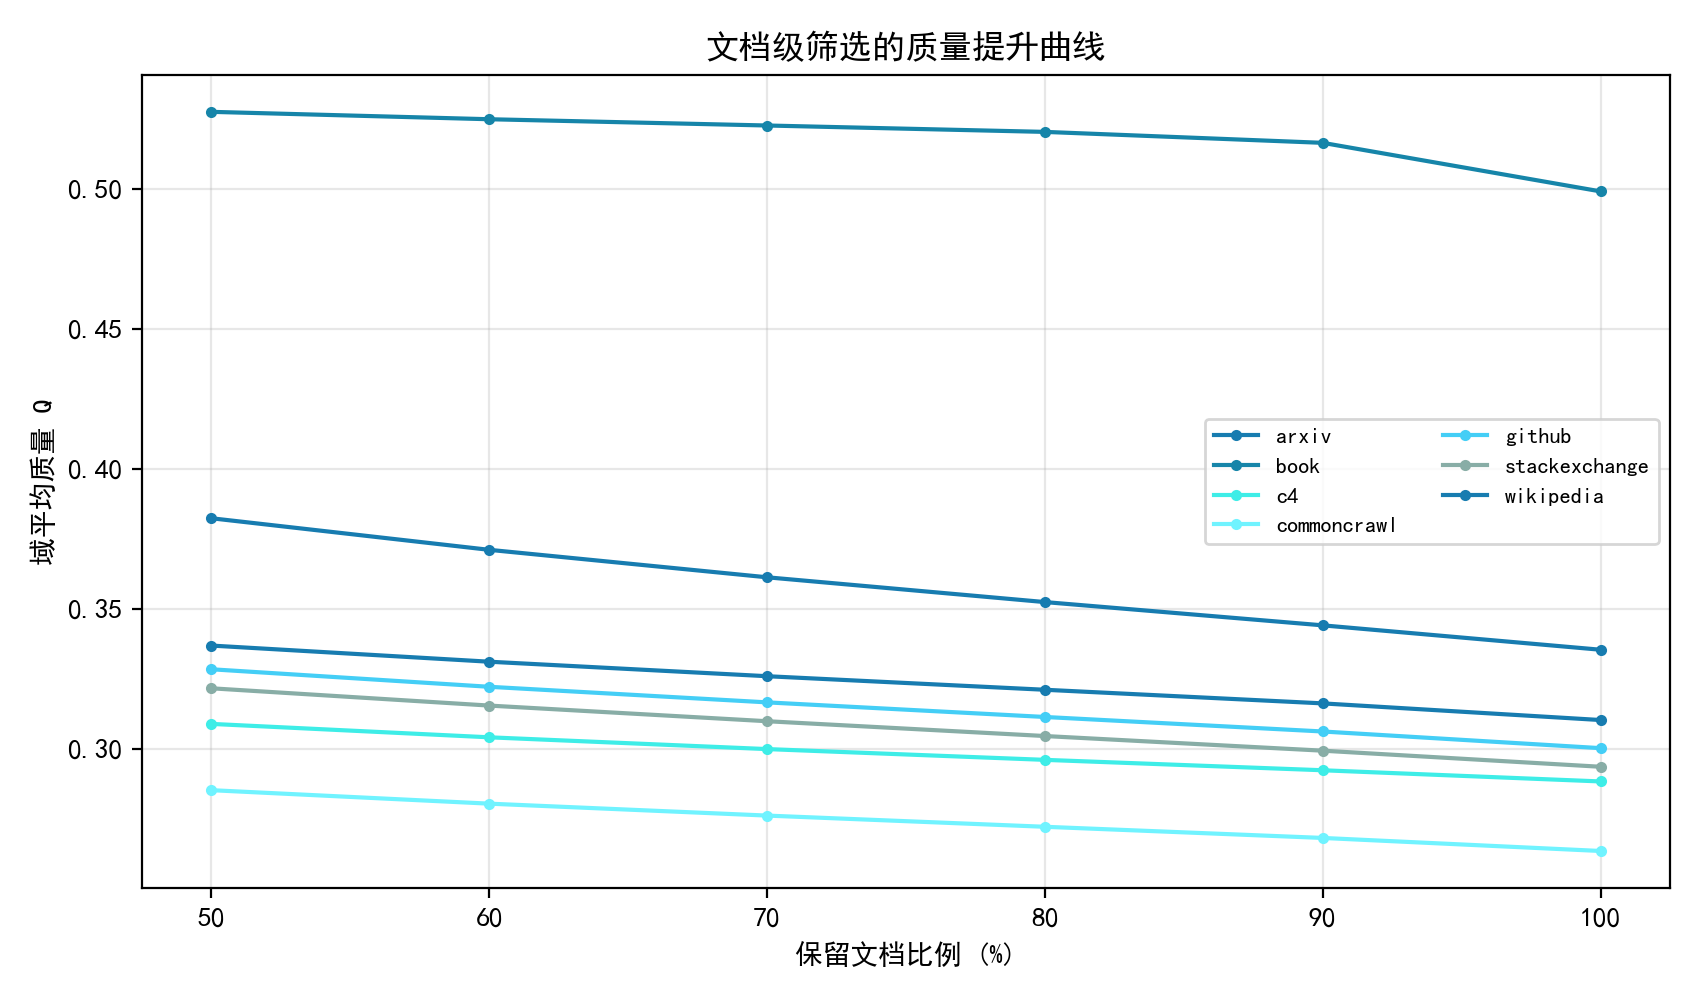
\includegraphics[width=0.8\textwidth]{figures/v60_p1_filter_curve.png}
\caption{文档级筛选的质量提升曲线：全域 3\%--5\%（arxiv/book 相对最大）。}
\label{fig:p1_filtercurve}
\end{figure}

\textbf{域画像的相似性结构}（图 \ref{fig:p1_domainprof}）：把每域的
22 维指标均值当作``域画像''，其相关矩阵呈\textbf{两极结构}：
\textbf{book 画像独树一帜}——与 github 相关仅 $-0.02$（近乎正交）、
与全部其他域 $\le 0.5$（最高 arxiv 0.49）；而低质通用域
c4/commoncrawl/stackexchange/wikipedia 两两相关 $\ge 0.82$，构成
\textbf{核心聚簇}；arxiv 居中（0.45--0.67）。含义：域序第一的 book
对应的是\textbf{画像的独特性}（质量高 = 画像不同），而非同一质量轴的
更高取值——与 v48 的 book 优势主要来自结构/格式族、v58 的分布形状
差异互相咬合。

\begin{figure}[htbp]
\centering
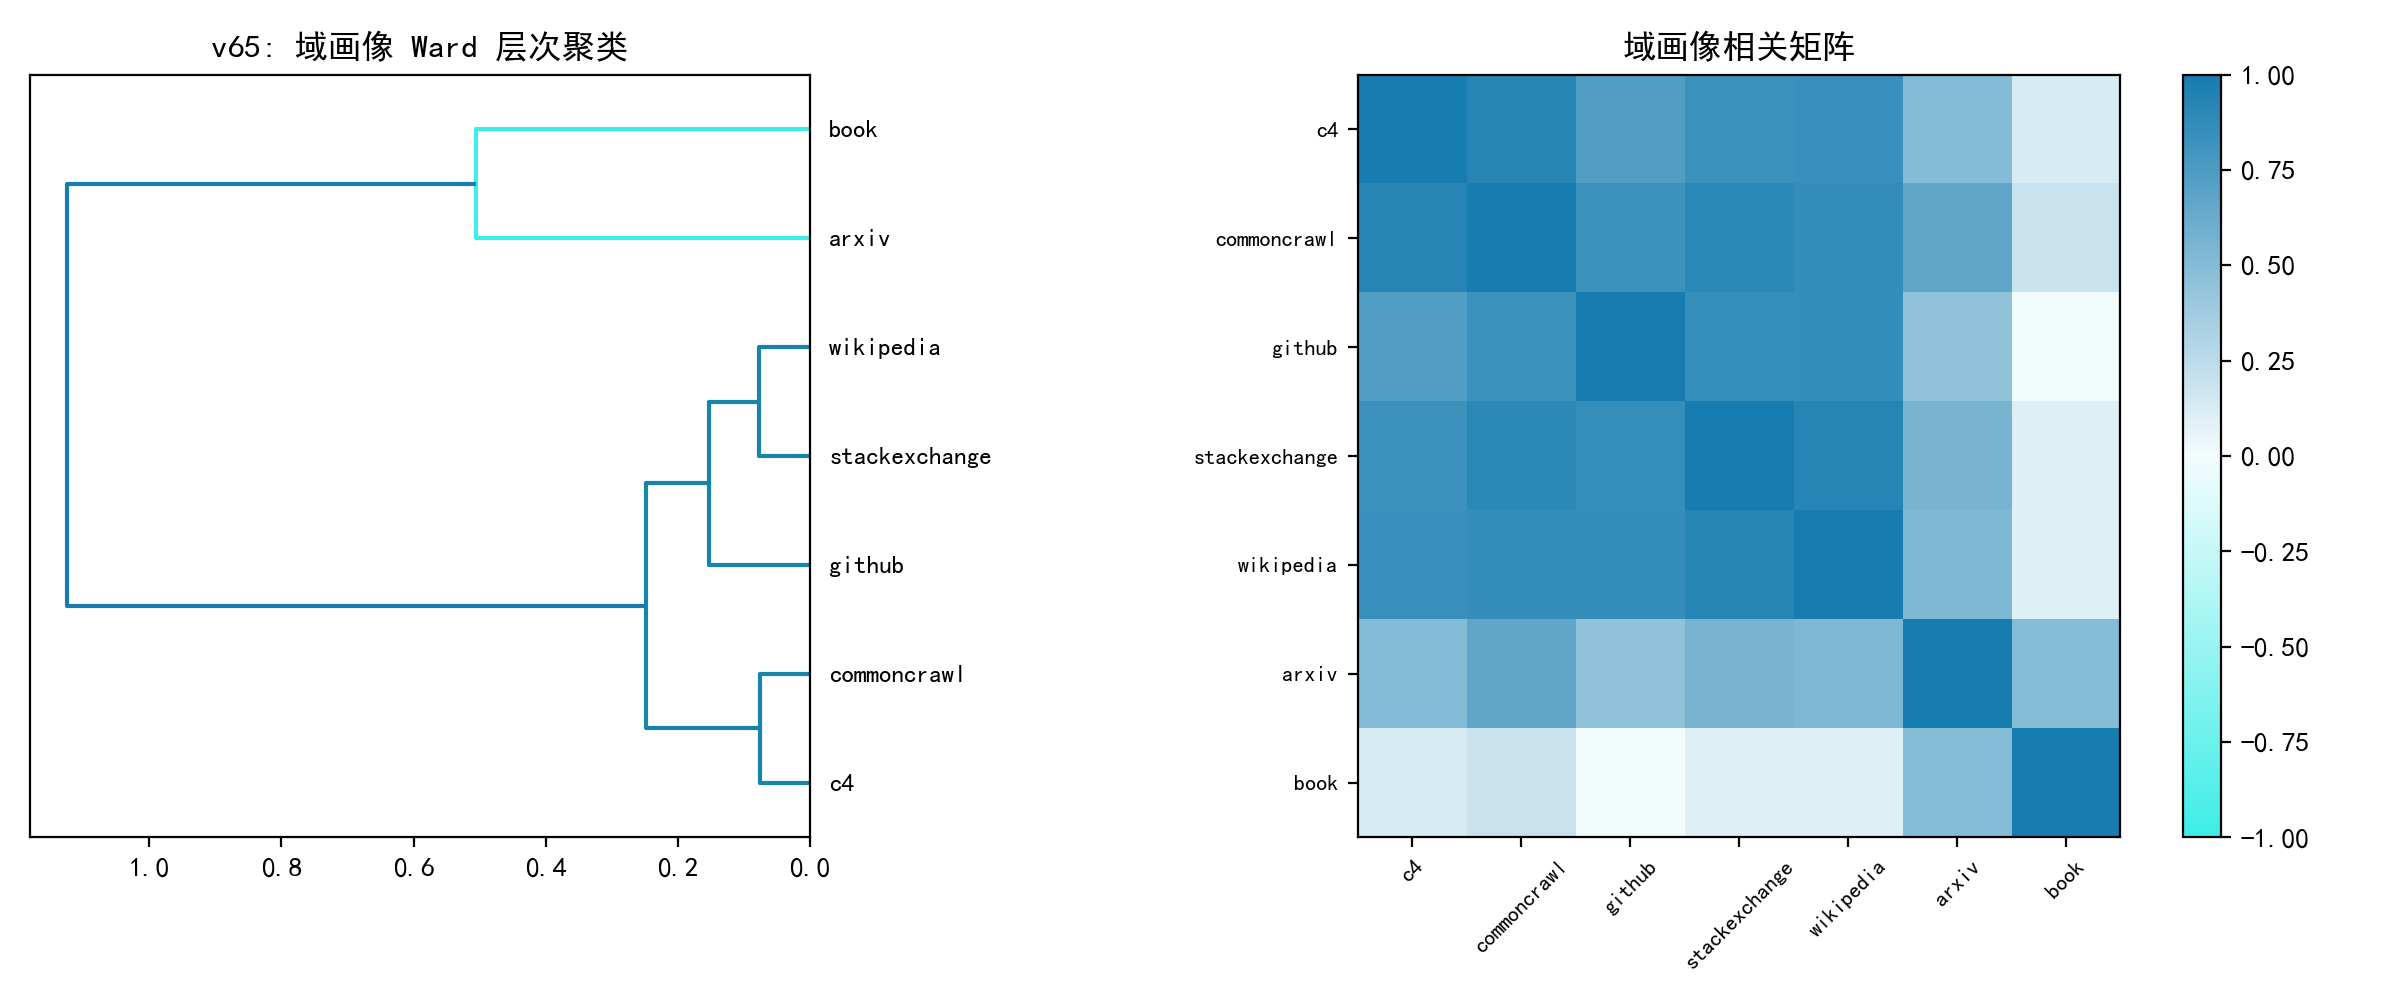
\includegraphics[width=0.92\textwidth]{figures/v65_p1_domain_prof.png}
\caption{域画像层次聚类与相关矩阵：book 独树一帜、低质域聚簇。}
\label{fig:p1_domainprof}
\end{figure}

\textbf{book 领先的指标族分解}（图 \ref{fig:p1_contrib}）：把加权标准化值
$V_{ij}=w_jX_{ij}$ 的域均值差按指标族可加分解，book 相对全域的加权分优势
为 0.1441，其中\textbf{结构/格式族贡献 +0.178}（主导），语义模型分族
$-0.013$ 与内容/主题族 $-0.021$ 近零。逐指标 Top5（词数 +0.084、句数
+0.077、大写字母比例 +0.027、句读结尾 +0.015、unigram 熵 +0.009）全部
为结构格式信号；commoncrawl 的负贡献则集中在大写比例（$-0.013$）与广告
类信号（$ad\_en=-0.007$）。这一分解说明：book 的领先主要来自
\textbf{长文档、规范句读、大写比例等结构性形式信号}，而非语义内容分——
结构性信号是域级质量判别的统计主体。

\begin{figure}[htbp]
\centering
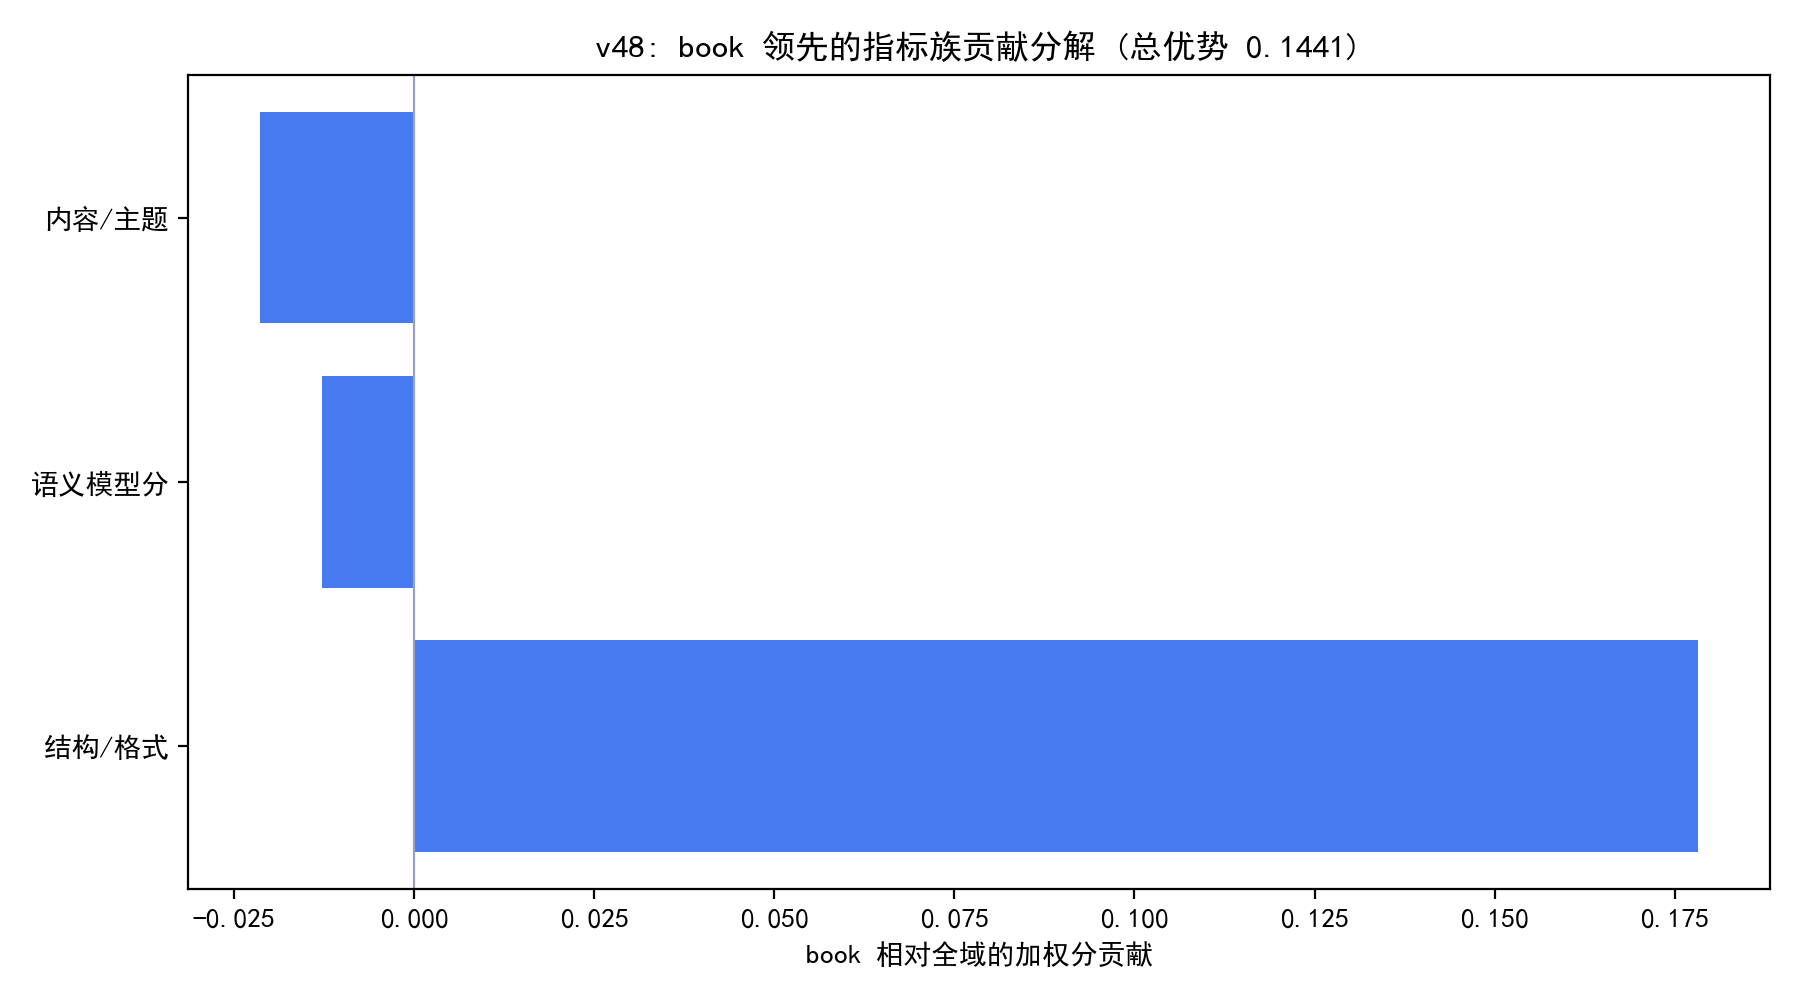
\includegraphics[width=0.8\textwidth]{figures/v48_p1_family_contrib.png}
\caption{book 领先的指标族贡献分解：结构/格式族主导。}
\label{fig:p1_contrib}
\end{figure}

\textbf{指标体系的有效维度}（图 \ref{fig:p1_pcadim}）：对 22 个指标
做 PCA，累积方差 50\%/80\%/90\% 分别只需 \textbf{3/8/11} 个主成分——
指标体系\textbf{冗余度高但非单维}（PC1 仅解释 34.2\%，PC1--6 累积
74.3\%）。载荷结构：PC1 是``内容质量''主成分（88\% 载荷来自内容族，
两族平均 |载荷| 0.230 vs 0.069）；格式洁净信息主要在 PC2/PC3
（两族载荷互补 0.186/0.145 与 0.170/0.175）。含义：两族信息
\textbf{正交互补、缺一不可}——若只用内容族指标会丢掉 book 优势所在的
独立信息轴（与 v48 的格式族主导互证），若只用格式族则会丢失 PC1 的
主信息。

\begin{figure}[htbp]
\centering
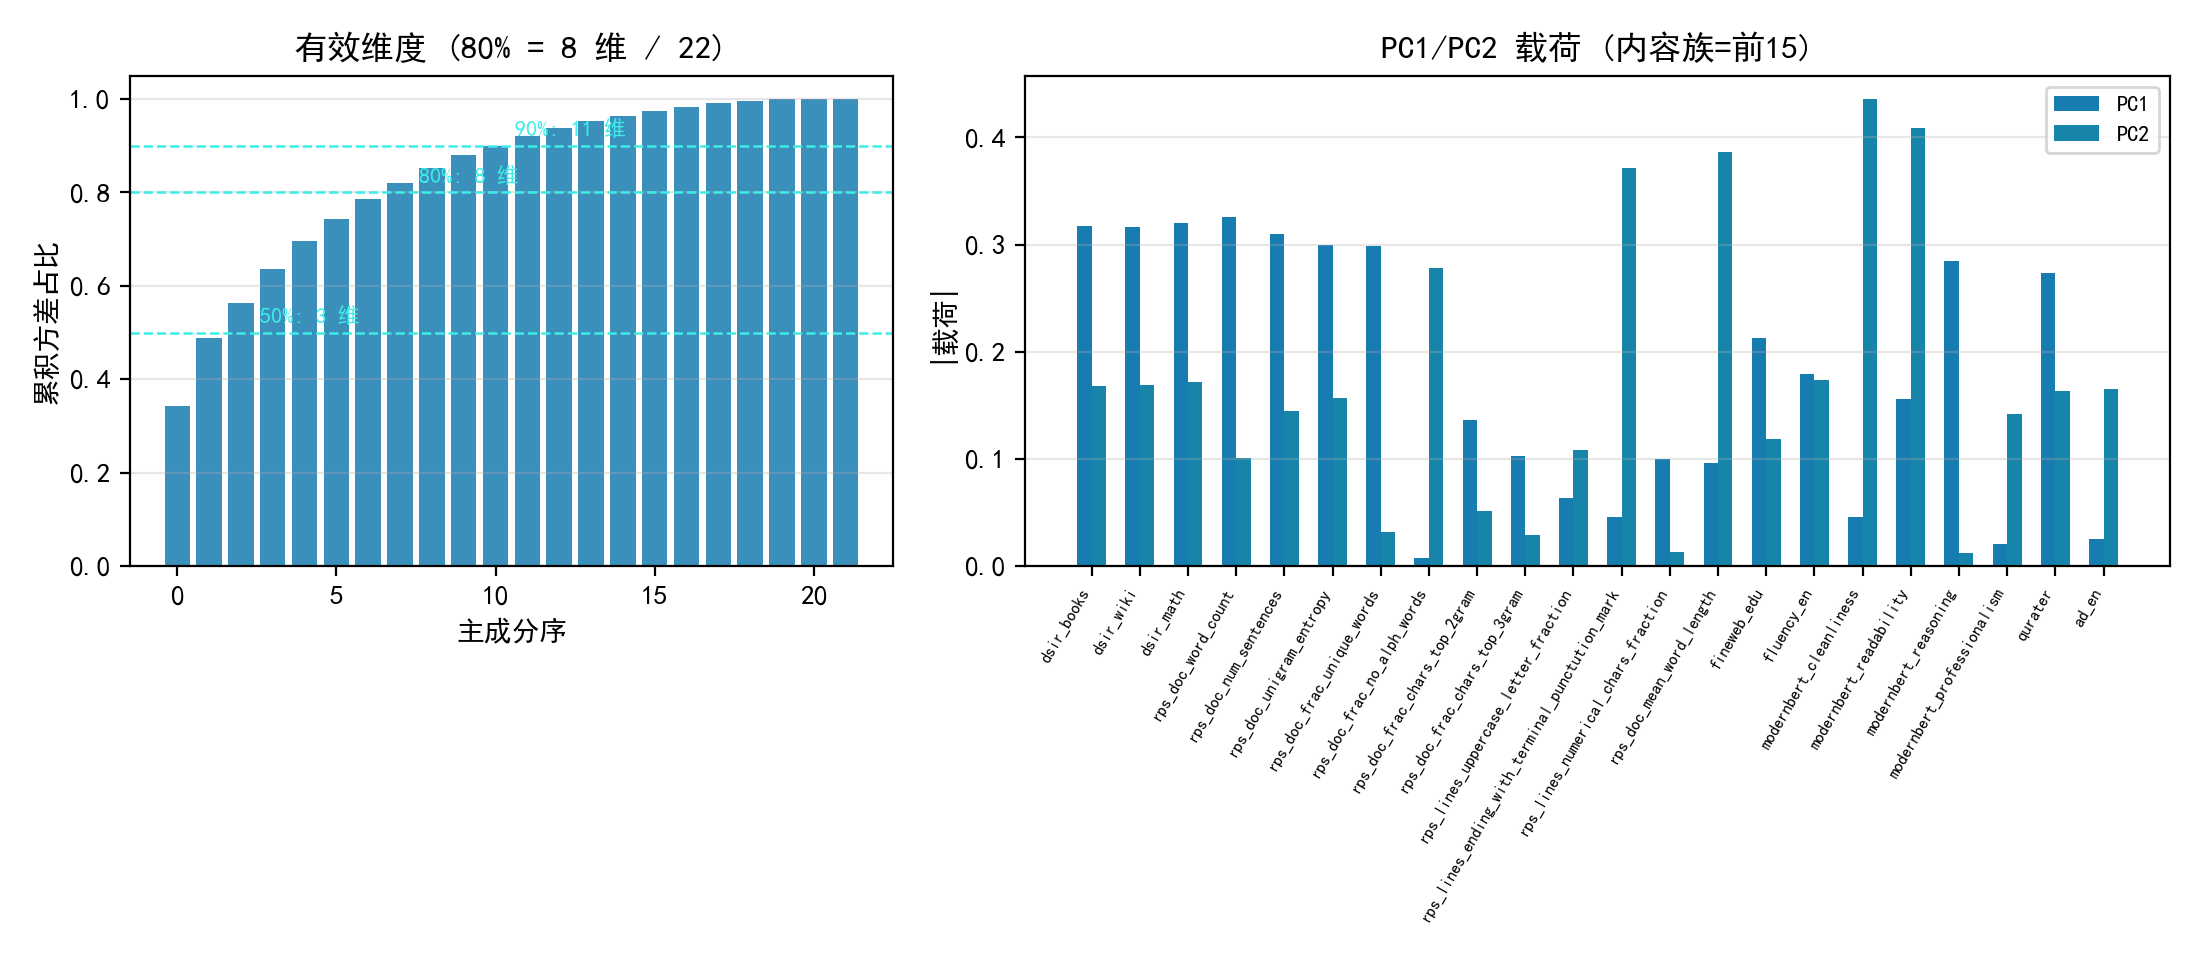
\includegraphics[width=0.92\textwidth]{figures/v70_p1_pca_dim.png}
\caption{22 指标的有效维度（80\%=8 维）与 PC1/PC2 载荷：两族互补。}
\label{fig:p1_pcadim}
\end{figure}

\subsubsection{抽样/全量一致性验证}

将 1M 抽样集与 A2/A3 扩展集合并后重新聚合，arxiv 域抽样口径 0.481 对全量
0.486、github 0.386 对 0.386，偏差均小于 0.005，说明 22 指标评分在抽样集
上训练、可安全迁移到全量扩展集，评分体系具有可迁移性。

\subsection{小结}

问题一建立了``预处理 $\to$ 组合赋权 $\to$ TOPSIS''的质量评分链，定义了
双族冲突指数并给出对称截尾消解规则，得到 7 域质量分；进一步用岭回归刻画
17 域配比与 13 损失域的数量关系，并通过跨尺度系数收缩（$\kappa=0.314$）
揭示了配比效应随规模递减的规律。质量分 $Q$ 与配比关系将作为问题二、三的
输入。
